% =====================================================================
%  NeuroBridge -- MSc Project Report
%  Compile with pdflatex (Overleaf default). Run twice for the contents.
%  Edit the names and roll numbers in the \teammember lines below.
% =====================================================================
\documentclass[11pt,a4paper]{article}

\usepackage[T1]{fontenc}
\usepackage[utf8]{inputenc}
\usepackage{lmodern}
\usepackage[a4paper,margin=2.5cm,headheight=14pt]{geometry}
\usepackage{amsmath,amssymb}
\usepackage{booktabs,tabularx,array,longtable}
\usepackage{enumitem}
\usepackage[table]{xcolor}
\usepackage{float}
\usepackage{caption}
\usepackage{fancyhdr}
\usepackage{listings}
\usepackage{tikz}
\usetikzlibrary{arrows.meta,positioning,shapes.geometric,shapes.misc,fit,calc,backgrounds}
\usepackage{pgfplots}
\pgfplotsset{compat=1.18}
\usepackage{chngcntr}
\usepackage[hidelinks]{hyperref}

\hypersetup{pdftitle={NeuroBridge: An AI-Powered Support Platform for Neurodivergent People and Their Caregivers},
            pdfauthor={Lisa Luis, Muskan Aga, Shannon Coelho (Group Maple), Goa University}}

% ---------- numbering per section, as in the example report ----------
\counterwithin{figure}{section}
\counterwithin{table}{section}
\captionsetup{font=small,labelfont=bf,skip=6pt}
\captionsetup[lstlisting]{justification=raggedright,singlelinecheck=false}
\setlist{itemsep=2pt,topsep=4pt}
\setlength{\parindent}{0pt}
\setlength{\parskip}{6pt}

% ---------- running header: "Chapter N. Title" ----------
\pagestyle{fancy}
\fancyhf{}
\fancyhead[L]{\small\nouppercase{\leftmark}}
\fancyfoot[C]{\thepage}
\renewcommand{\headrulewidth}{0.4pt}
\newif\ifinappendix
\renewcommand{\sectionmark}[1]{\markboth{\ifinappendix Appendix\else Chapter\fi\ \thesection.\ \ #1}{}}

% ---------- colours ----------
\definecolor{nbteal}{HTML}{2E7D73}
\definecolor{nbgreen}{HTML}{E8F5E9}
\definecolor{nbgreenD}{HTML}{4C8C4A}
\definecolor{nbgray}{HTML}{EEEEEE}
\definecolor{nbgrayD}{HTML}{7A7A7A}
\definecolor{nborange}{HTML}{FFF3E0}
\definecolor{nborangeD}{HTML}{D08A2E}
\definecolor{nbpink}{HTML}{FCE4EC}
\definecolor{nbpinkD}{HTML}{B0577A}
\definecolor{nbblue}{HTML}{E3F2FD}
\definecolor{nbblueD}{HTML}{4A7FB0}
\definecolor{nblav}{HTML}{EDE7F6}
\definecolor{nblavD}{HTML}{7E62B3}
\definecolor{codebg}{HTML}{F7F7F7}
\definecolor{codekw}{HTML}{1F5F99}
\definecolor{codestr}{HTML}{A0522D}
\definecolor{codecom}{HTML}{6A8759}

% ---------- TikZ styles ----------
\tikzset{
  base/.style={draw, rounded corners=3pt, align=center, font=\small, inner sep=5pt, line width=0.6pt},
  green/.style={base, fill=nbgreen, draw=nbgreenD},
  gray/.style={base, fill=nbgray, draw=nbgrayD},
  orange/.style={base, fill=nborange, draw=nborangeD},
  pink/.style={base, fill=nbpink, draw=nbpinkD},
  blue/.style={base, fill=nbblue, draw=nbblueD},
  lav/.style={base, fill=nblav, draw=nblavD},
  plain/.style={base, fill=white, draw=nbgrayD},
  decision/.style={diamond, aspect=2.2, draw=nbblueD, fill=nbblue, font=\small, align=center, inner sep=1pt, line width=0.6pt},
  arr/.style={-{Stealth[length=2.2mm]}, draw=nbgrayD, line width=0.6pt},
  darr/.style={arr, dashed},
  lbl/.style={font=\footnotesize, text=black!70},
  group/.style={draw=nbgrayD, dashed, rounded corners=4pt, inner sep=8pt},
}

% ---------- code listings ----------
\lstdefinestyle{nb}{
  backgroundcolor=\color{codebg},
  basicstyle=\ttfamily\footnotesize,
  keywordstyle=\color{codekw}\bfseries,
  stringstyle=\color{codestr},
  commentstyle=\color{codecom}\itshape,
  frame=single, rulecolor=\color{black!15},
  breaklines=true, breakatwhitespace=true,
  showstringspaces=false, tabsize=4, columns=fullflexible, keepspaces=true,
  numbers=left, numberstyle=\tiny\color{black!40}, numbersep=6pt,
  xleftmargin=14pt, framexleftmargin=14pt,
  aboveskip=8pt, belowskip=4pt,
  captionpos=b,
}
\lstset{style=nb, language=Python}
\renewcommand{\lstlistingname}{Listing}
\renewcommand{\lstlistlistingname}{List of Listings}
\AtBeginDocument{\counterwithin{lstlisting}{section}}
\newcommand{\code}[1]{\texttt{#1}}
\newcolumntype{Y}{>{\raggedright\arraybackslash}X}
\newcolumntype{L}[1]{>{\raggedright\arraybackslash}p{#1}}

% ---------- title-page team (EDIT HERE) ----------
\newcommand{\teamrows}{%
  Lisa Luis & 25P0620008\\
  Muskan Aga & 25P0620011\\
  Shannon Coelho & 25P0620019\\
}

\begin{document}

% =====================================================================
%  TITLE PAGE
% =====================================================================
\begin{titlepage}
\centering
\vspace*{1.2cm}
{\large\bfseries GOA UNIVERSITY\par}
\vspace{0.3cm}
{\normalsize MSc Artificial Intelligence\par}
\vspace{1.8cm}
{\LARGE\bfseries NeuroBridge: An AI-Powered Support Platform\\[4pt] for Neurodivergent People and Their Caregivers\par}
\vspace{0.9cm}
{\normalsize A Consent-Based Web Application with a Source-Verified Research Agent,\\
a Rule-Based Safety Layer and a QLoRA SFT / ORPO Fine-Tuning Pipeline\par}
\vspace{2.2cm}
{\Large\bfseries PROJECT REPORT\par}
\vspace{1.6cm}
{\normalsize Submitted by Group Maple\par}
\vspace{0.5cm}
\begin{tabular}{ll}
\textbf{Name} & \textbf{Roll Number}\\[2pt]
\teamrows
\end{tabular}
\vspace{2.2cm}

{\bfseries Programme: MSc in Artificial Intelligence\par}
\vfill
{\normalsize November 2026\par}
\end{titlepage}

\pagenumbering{roman}
\setcounter{page}{1}
\markboth{Abstract}{}

% =====================================================================
%  ABSTRACT
% =====================================================================
\section*{Abstract}
\addcontentsline{toc}{section}{Abstract}

Neurodivergent people and the families who support them often manage routines, appointments,
sensory needs and communication across many unconnected tools, while general-purpose chatbots
can give confident answers that are unsourced, incomplete or unsafe. This project builds
\textbf{NeuroBridge}, a working web application that brings daily support, consent-based care
coordination, a moderated peer community and an AI assistant together in one place.

The assistant joins two components. A conversational language model handles everyday help, and
a research agent plans, calls tools, reads web pages, verifies its claims against the sources
it retrieved, and asks the user for approval before any booking. A rule-based safety layer answers
emergencies, self-harm and acute psychosis with fixed, sourced guidance that never passes
through a language model. Caregivers see only what the individual explicitly shares, scope by scope,
and private journals, AI memory and AI conversations can never be shared.

The system has three parts: a FastAPI web application with 43 database tables and about 130
authenticated endpoints; the research agent with deterministic evidence checks; and a
reproducible pipeline that fine-tunes Qwen2.5-1.5B-Instruct with QLoRA supervised fine-tuning
(SFT) and, as a labelled ablation, Odds Ratio Preference Optimization (ORPO).

An audit of the inherited 12,000-row training set found that it held only 768 unique
instructions and that its responses were assembled from 164 distinct lines; 25\% contained a
leaked instruction and 96\% a broken sentence splice. The pipeline therefore measures templating,
repairs what it can and separates evidence that a model has \emph{learned} the data from evidence
that its answers are \emph{better}.

All 158 automated tests passed from a clean copy of the code, and every page was checked in a headless
browser and for colour contrast. The fine-tuned models have not yet been trained at full scale or rated by
people, so this report makes no claim that SFT or ORPO improves answer quality.

\textbf{Keywords:} Neurodiversity, Assistive Technology, Large Language Models, LLM Agents,
Retrieval-Augmented Generation, QLoRA, ORPO, Consent, AI Safety, FastAPI.

\clearpage
\markboth{Contents}{}
\tableofcontents
\clearpage
\markboth{Lists of Figures, Tables and Listings}{}
\listoffigures
\listoftables
\lstlistoflistings
\clearpage

\pagenumbering{arabic}
\setcounter{page}{1}

% =====================================================================
\section{Introduction}
% =====================================================================

\subsection{Background}
Neurodivergence covers natural differences in how people think, sense and communicate, such as
autism, ADHD, dyslexia, dyspraxia and sensory processing differences. Many neurodivergent people
find everyday tasks such as starting a task, switching between activities, coping with noise or explaining what they
need harder in environments built for others. Parents, partners and support workers often help,
but coordinating that help without taking control away from the person is difficult.

Large Language Models (LLMs) can hold helpful conversations, plan tasks and summarise information.
However, a general model may invent facts, links or organisations, give answers that are too long
for someone who is overwhelmed, or respond poorly in an emergency. An \emph{agent} adds tool use, so
the model can search the web or book an event. That makes it more useful but also raises the stakes.

\subsection{Problem Statement}
There was no single, neurodiversity-affirming tool in which an individual and their chosen
supporters can plan, communicate and find help, where:
\begin{itemize}
  \item the individual controls exactly what each supporter can see;
  \item factual answers are backed by sources that the user can check;
  \item consequential actions such as bookings happen only with explicit approval; and
  \item emergencies are handled reliably, without depending on what a language model happens to generate.
\end{itemize}
A second problem was inherited: an earlier fine-tuning attempt had used a 12,000-row dataset
whose quality had never been measured.

\subsection{Aim}
To design, build and test a full-stack web application, NeuroBridge, that joins a conversational LLM
and a research agent under consent, approval and safety rules enforced in code. A second aim was to build a
reproducible pipeline for fine-tuning and honestly evaluating a small NeuroBridge model.

\subsection{Objectives}
\begin{enumerate}
  \item Audit the two earlier project notebooks (agent prototype and LLM training) and keep what worked.
  \item Complete the research agent: planning, tool execution, web reading, verification, correction, replanning and goal checks.
  \item Build two distinct experiences, individual and caregiver, connected by explicit and revocable consent.
  \item Add Community Connect: interest groups, peer connections, events and clubs, with moderation and protections for minors.
  \item Build a safety layer for emergencies, self-harm, psychosis and requests for diagnosis or medication changes.
  \item Build a dataset-curation, QLoRA SFT and gated ORPO pipeline, with an evaluation that separates learning from quality.
  \item Test every component, report the results honestly and document how to run the system.
\end{enumerate}

\subsection{Research Questions}
\begin{enumerate}[label=\textbf{RQ\arabic*.}]
  \item Can a single web application connect a chat LLM and a tool-using agent while giving each one only the context the user has permitted?
  \item Can safety, consent and approval rules be enforced in code, so that they hold whichever language model is used?
  \item What can the inherited 12,000-row dataset show about learning and quality when a small model is fine-tuned on it?
\end{enumerate}

\subsection{Project Scope}
NeuroBridge is a support tool, not a medical service. It does not diagnose conditions, recommend
medication changes, provide crisis counselling or make emergency decisions on anyone's behalf. It is an
academic prototype that has not been clinically validated or tested with real users, and no
compliance with GDPR, India's Digital Personal Data Protection Act or HIPAA is claimed.

\subsection{Organisation of the Report}
Chapter~\ref{sec:related} reviews related work and Chapter~\ref{sec:background} explains the technical
background. Chapter~\ref{sec:requirements} sets out requirements and ethical design, and
Chapter~\ref{sec:architecture} the system architecture. Chapters~\ref{sec:webapp}--\ref{sec:safety}
describe the web application, the AI assistant and agent, and the safety layer.
Chapter~\ref{sec:llm} covers the dataset audit and fine-tuning pipeline. Chapter~\ref{sec:testing}
reports testing, Chapter~\ref{sec:ethics} discusses ethics and limitations, and
Chapter~\ref{sec:conclusion} concludes. The appendices give run instructions, environment
variables, an API summary and the safety probe categories.

% =====================================================================
\section{Related Work}\label{sec:related}
% =====================================================================

\subsection{Neurodiversity-Affirming Support Tools}
The neurodiversity paradigm treats neurological differences as natural variation rather than
defects to be cured. For software this means centring the person's own preferences and goals,
never making compliance or ``masking'' the target, and giving supporters coordination tools rather than
surveillance. Accessibility guidance such as WCAG~2.2~\cite{wcag22} covers many of the needs, including
keyboard use, contrast and reduced motion. Cognitive and sensory load also matter: a calm layout, short
sentences and one choice at a time.

\subsection{Conversational Agents and Tool Use}
Instruction-tuned LLMs follow requests well after alignment with human feedback~\cite{ouyang2022}.
Retrieval-augmented generation (RAG)~\cite{lewis2020} conditions an answer on retrieved documents
to reduce unsupported claims. Agent frameworks such as ReAct~\cite{yao2022} interleave reasoning with
tool calls. NeuroBridge combines both ideas. It then adds a deterministic verification step: every URL, phone
number, price and organisation name in an answer must appear in a retrieved source, or it is removed.

\subsection{Parameter-Efficient Fine-Tuning}
LoRA~\cite{hu2022} trains small low-rank updates instead of all weights, and QLoRA~\cite{dettmers2023}
stores the frozen model in 4-bit precision so that billion-parameter models can be fine-tuned on a
single consumer GPU. The Qwen2.5 family~\cite{qwen25report,qwenhf} includes a 1.5-billion-parameter
instruction model that fits a free Colab T4 GPU when quantised.

\subsection{Preference Optimization}
Reinforcement learning from human feedback uses a separate reward model~\cite{ouyang2022}. Direct
Preference Optimization~\cite{rafailov2023} removes the reward model but still needs a frozen reference
model. ORPO~\cite{hong2024} adds an odds-ratio penalty on rejected responses to the ordinary SFT loss,
so it needs neither. The ORPO paper reports results with large, diverse preference datasets; its
behaviour with a few hundred automatically built pairs is not established.

\subsection{Safety in Mental-Health AI}
A support assistant will meet emergencies, self-harm and acute psychosis. Generated text can be
wrong, cut off or too long at exactly those moments. In India, 112 is the national emergency number and
Tele-MANAS offers free 24$\times$7 tele-mental-health support on 14416 or 1-800-891-4416~\cite{telemanas}.
First-aid steps for choking, CPR, seizures, stroke and bleeding are published by the NHS, CDC,
Resuscitation Council UK and the British Red Cross~\cite{nhs,cdc,resus,redcross}.

\subsection{Position of This Work}
This work does not propose a new learning method. Its contribution is engineering and evaluation:
a working platform in which consent, approval and safety are enforced in code and covered by tests,
together with an honest audit of the training data and an evaluation design that does not overclaim.

% =====================================================================
\section{Technical Background}\label{sec:background}
% =====================================================================

\subsection{Qwen2.5-1.5B-Instruct}
The base model for fine-tuning is \code{Qwen/Qwen2.5-1.5B-Instruct}~\cite{qwenhf,qwen25report}, an
open-weight instruction model with about 1.5 billion parameters. It is small enough to train with
QLoRA and to serve on a free Colab Tesla T4 GPU. For everyday use the application can also call hosted
models through Groq or Gemini API keys.

\subsection{Supervised Fine-Tuning (SFT)}
In SFT the model is trained on pairs of an input and a desired output, which makes the desired
output more likely token by token. NeuroBridge computes the loss on the \emph{response only}: the
system prompt and user message are masked so the model is not trained to repeat them.

\begin{quote}\small
\textbf{System:} You are NeuroBridge, a neurodiversity-affirming support assistant\ldots\\
\textbf{User:} I have to clean my room and I can't start.\\
\textbf{Assistant:} Let's make it small. Pick up five things near you --- that's all for now. Tell me when you're done and we can choose the next tiny step.
\end{quote}
This is an illustrative example of the format, not a record from the dataset.

\subsection{LoRA and QLoRA}
LoRA keeps the original weight matrix $W$ frozen and learns an update $\Delta W = BA$, where
$B\in\mathbb{R}^{d\times r}$ and $A\in\mathbb{R}^{r\times k}$ have a small rank $r$:
\begin{equation}
  h = Wx + \frac{\alpha}{r}\,BAx .
\end{equation}
This project uses rank $r=16$ and scaling $\alpha=32$ on all attention and MLP projection layers.
QLoRA stores $W$ in 4-bit NF4 format with double quantization, while only $A$ and $B$ are trained
in 16-bit precision.

\begin{figure}[H]
\centering
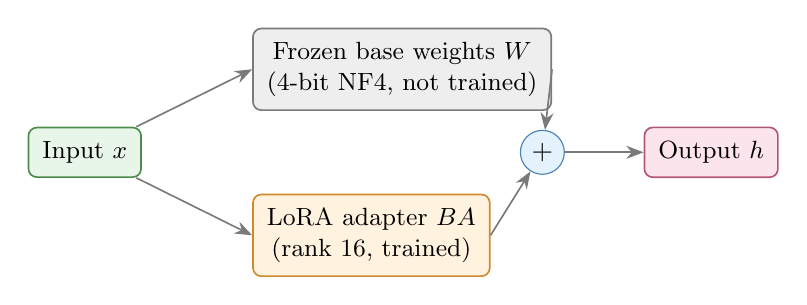
\begin{tikzpicture}[node distance=6mm and 12mm]
  \node[green] (in) {Input $x$};
  \node[gray, above right=2mm and 14mm of in] (w) {Frozen base weights $W$\\(4-bit NF4, not trained)};
  \node[orange, below right=2mm and 14mm of in] (ab) {LoRA adapter $BA$\\(rank 16, trained)};
  \node[circle, draw=nbblueD, fill=nbblue, right=48mm of in, inner sep=2pt] (plus) {$+$};
  \node[pink, right=10mm of plus] (out) {Output $h$};
  \draw[arr] (in) -- (w.west);
  \draw[arr] (in) -- (ab.west);
  \draw[arr] (w.east) -- (plus);
  \draw[arr] (ab.east) -- (plus);
  \draw[arr] (plus) -- (out);
\end{tikzpicture}
\caption{How a LoRA adapter works: the input passes through the frozen 4-bit weights and through the small trained adapter, and the two results are added.}
\label{fig:lora}
\end{figure}

\subsection{Odds Ratio Preference Optimization (ORPO)}
Each ORPO record has a prompt $x$, a chosen response $y_w$ and a rejected response $y_l$. With
$\mathrm{odds}_\theta(y\mid x) = \frac{P_\theta(y\mid x)}{1-P_\theta(y\mid x)}$, the loss is
\begin{equation}
  \mathcal{L}_{\text{ORPO}} = \mathcal{L}_{\text{SFT}}(y_w)
  \;-\; \lambda \,\log\sigma\!\left(\log\frac{\mathrm{odds}_\theta(y_w\mid x)}{\mathrm{odds}_\theta(y_l\mid x)}\right),
\end{equation}
where $P_\theta$ is the length-normalised sequence likelihood and $\lambda=0.1$. The first term keeps
the model close to the preferred answers; the second pushes the chosen answer above the rejected one.
No frozen reference model is needed, which keeps memory use low.

\subsection{Retrieval, Agents and Verification}
A \emph{tool} is a function the agent may call, such as web search, page reading, event search or
registration. The agent \emph{plans} which tools to call, \emph{executes} them, \emph{observes} the
results, drafts an answer citing numbered sources (S1, S2,~\ldots), and then \emph{verifies} that answer
against what it actually retrieved before showing it to the user.

\subsection{Key Terms}
\begin{table}[H]
\centering
\caption{Glossary of terms used in the report}
\label{tab:glossary}
\small
\begin{tabularx}{\textwidth}{@{}lY@{}}
\toprule
\textbf{Term} & \textbf{Meaning}\\
\midrule
Token & A small piece of text (a word or part of a word) that the model reads and writes.\\
Adapter & The small set of trained LoRA weights that sits on top of the frozen base model.\\
Agent & A program in which an LLM plans and calls tools, observes results and decides what to do next.\\
Tool & A function the agent may call, for example web search or event registration.\\
Grounding & Checking that each factual claim in an answer is supported by a retrieved source.\\
Redaction & Removing unsupported statements from an answer before it is shown.\\
Approval hash & A SHA-256 fingerprint of the exact details a user approved; a booking fails if they change.\\
Scope & One category of data an individual may share with a caregiver, such as routines or calendar.\\
Templated data & Training text assembled from a few repeated sentences rather than written individually.\\
Ablation & A run carried out to study an effect, labelled so it is not mistaken for a validated model.\\
Endpoint & A URL on the server that the interface calls to read or change data.\\
\bottomrule
\end{tabularx}
\end{table}

% =====================================================================
\section{Requirements and Ethical Design}\label{sec:requirements}
% =====================================================================

\subsection{User Groups}
\begin{table}[H]
\centering
\caption{User groups, their needs and what they must never get}
\label{tab:users}
\small
\begin{tabularx}{\textwidth}{@{}L{3.6cm}YY@{}}
\toprule
\textbf{Group} & \textbf{Main needs} & \textbf{Must never get}\\
\midrule
Neurodivergent individuals & Plan without pressure, communicate needs, calm down when overwhelmed, find community & Streaks, guilt or pressure; their journal exposed to anyone\\
Caregivers and supporters & Coordinate appointments and tasks, understand the person, look after themselves & Access the individual has not granted\\
Moderators / admins & Review held posts, reports and proposed events & Admin rights through self-registration\\
\bottomrule
\end{tabularx}
\end{table}

\subsection{Functional Requirements}
\begin{itemize}
  \item Accounts with individual, caregiver and admin roles, and separate navigation for each.
  \item Daily support: My Day, tasks with small first steps, routines, check-ins, sensory toolkit, communication cards, journal, Support Blueprint and goals.
  \item Caregiver tools: dashboard, care journal, care calendar, coordination, support requests and wellbeing.
  \item An AI assistant that chats, researches with citations, and books events or appointments only after approval.
  \item Community Connect: interest groups, posts, peer connections, private messages, events and clubs.
  \item A one-tap \emph{I'm overwhelmed} mode on every page.
\end{itemize}

\subsection{Non-Functional Requirements}
\begin{itemize}
  \item \textbf{Privacy:} data isolated per user; caregivers see only what is explicitly shared; data export and real deletion.
  \item \textbf{Honesty:} no invented sources, bookings or confirmations; failures are shown as failures.
  \item \textbf{Accessibility:} keyboard use, screen readers, reduced motion, high contrast, dyslexia-friendly font, low-stimulation mode, text-to-speech and speech-to-text.
  \item \textbf{Deployability:} runs in Google Colab, the only available environment, with all secrets from environment variables.
\end{itemize}

\subsection{From Ethical Principles to Code}
\begin{table}[H]
\centering
\caption{Ethical principles and the rule that enforces each one}
\label{tab:ethics}
\small
\begin{tabularx}{\textwidth}{@{}L{3.4cm}Y@{}}
\toprule
\textbf{Principle} & \textbf{Rule in the system}\\
\midrule
Autonomy & A care link grants nothing until the individual turns on each sharing scope.\\
Privacy & Journal, AI memory and AI conversations can never be shared.\\
Non-maleficence & Emergencies get fixed first-aid text and 112; no LLM call in that path.\\
No diagnosis & Diagnosis and medication-change requests get a policy note and a referral.\\
Consent for action & Bookings bind approval to a hash of the exact title, time, place, fee and attendees.\\
Honesty about data & Synthetic training data is labelled; no claim of human validation.\\
Protection of minors & Under-18s use guardian mode, cannot be caregivers, and adults cannot message them privately.\\
\bottomrule
\end{tabularx}
\end{table}

% =====================================================================
\section{System Architecture}\label{sec:architecture}
% =====================================================================

\subsection{Overall Architecture}
NeuroBridge runs as a single FastAPI~\cite{fastapi} server that hosts the web application, the AI assistant and
the original agent API, so it starts with one command in Colab or on a laptop
(Figure~\ref{fig:arch}).

\begin{figure}[H]
\centering
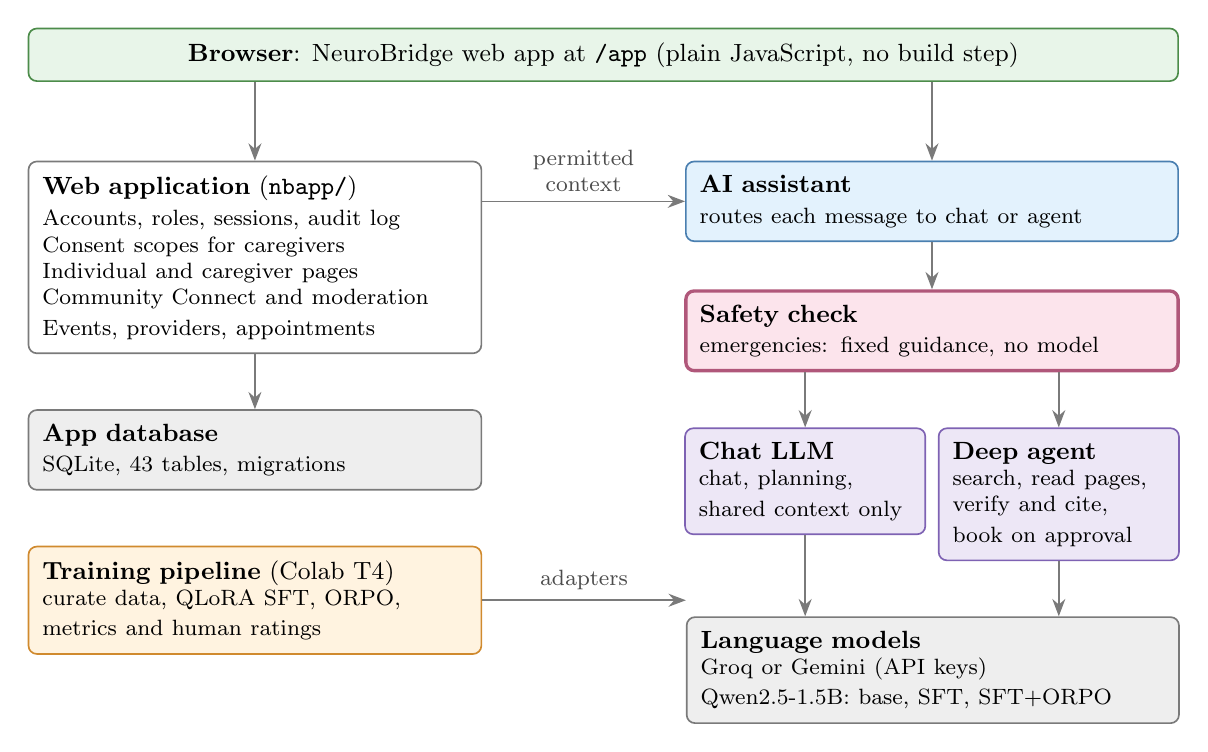
\begin{tikzpicture}[node distance=7mm, every node/.style={font=\small}]
  \node[green, minimum width=14.6cm] (browser) {\textbf{Browser}: NeuroBridge web app at \code{/app} (plain JavaScript, no build step)};

  \node[plain, below=10mm of browser.south west, anchor=north west, text width=5.4cm, align=left] (web)
    {\textbf{Web application} (\code{nbapp/})\\[2pt]
     \footnotesize Accounts, roles, sessions, audit log\\
     \footnotesize Consent scopes for caregivers\\
     \footnotesize Individual and caregiver pages\\
     \footnotesize Community Connect and moderation\\
     \footnotesize Events, providers, appointments};
  \node[gray, below=7mm of web, text width=5.4cm, align=left] (db)
    {\textbf{App database}\\ \footnotesize SQLite, 43 tables, migrations};
  \node[orange, below=7mm of db, text width=5.4cm, align=left] (train)
    {\textbf{Training pipeline} (Colab T4)\\ \footnotesize curate data, QLoRA SFT, ORPO,\\ \footnotesize metrics and human ratings};

  \node[blue, below=10mm of browser.south east, anchor=north east, text width=5.9cm, align=left] (asst)
    {\textbf{AI assistant}\\ \footnotesize routes each message to chat or agent};
  \node[pink, below=6mm of asst, text width=5.9cm, align=left, line width=1.2pt] (safe)
    {\textbf{Safety check}\\ \footnotesize emergencies: fixed guidance, no model};
  \node[lav, below=7mm of safe.south west, anchor=north west, text width=2.7cm, align=left] (chat)
    {\textbf{Chat LLM}\\ \footnotesize chat, planning,\\ \footnotesize shared context only};
  \node[lav, below=7mm of safe.south east, anchor=north east, text width=2.7cm, align=left] (agent)
    {\textbf{Deep agent}\\ \footnotesize search, read pages,\\ \footnotesize verify and cite,\\ \footnotesize book on approval};
  \node[gray, anchor=north east, text width=5.9cm, align=left] (models) at ($(agent.south east)+(0,-7mm)$)
    {\textbf{Language models}\\ \footnotesize Groq or Gemini (API keys)\\ \footnotesize Qwen2.5-1.5B: base, SFT, SFT+ORPO};

  \draw[arr] (browser.south -| web.north) -- (web.north);
  \draw[arr] (browser.south -| asst.north) -- (asst.north);
  \draw[arr] (web.east |- asst.west) -- node[lbl, above, align=center]{permitted\\context} (asst.west);
  \draw[arr] (web) -- (db);
  \draw[arr] (asst) -- (safe);
  \draw[arr] (safe.south -| chat.north) -- (chat.north);
  \draw[arr] (safe.south -| agent.north) -- (agent.north);
  \draw[arr] (chat.south) -- (chat.south |- models.north);
  \draw[arr] (agent.south) -- (agent.south |- models.north);
  \draw[arr] (train.east) -- node[lbl, above]{adapters} (train.east -| models.west);
\end{tikzpicture}
\caption{System architecture. One FastAPI server hosts the web application and the AI; every message passes the safety check before any model sees it.}
\label{fig:arch}
\end{figure}

\subsection{Architecture Explained Step by Step}
\begin{enumerate}
  \item \textbf{Browser.} The user signs in at \code{/app}. The interface is a single-page application written in plain JavaScript modules; it calls the server with a bearer token.
  \item \textbf{Web application.} FastAPI routers check the session, the role and, for caregivers, the consent scope before reading or writing any data.
  \item \textbf{AI assistant.} When the user sends a message, the web application passes only the context the user may see, such as their own preferences, memories (if switched on) or items an individual has shared.
  \item \textbf{Safety check.} The message is classified first. Emergencies, self-harm and crisis messages get fixed guidance and stop here.
  \item \textbf{Chat or agent.} Everyday requests go to the chat LLM. Requests that need sources, places, providers, events or bookings go to the research agent.
  \item \textbf{Models.} Both use one gateway that can call Groq, Gemini or the local NeuroBridge models produced by the training pipeline.
\end{enumerate}

\subsection{Stack Decision}
The inherited project already used FastAPI, SQLite and a plain-JavaScript console. Migrating to
React and PostgreSQL was considered. The project brief allowed migration only if the existing architecture was
unsuitable, and it was suitable. A Node.js build step would also add a fragile dependency in Colab, the only
environment available. The stack was therefore kept and extended: FastAPI routers (\code{nbapp/})
mounted on the existing app, and a modular plain-JavaScript interface. All SQL sits inside one
\code{Database} class, so a later move to PostgreSQL is contained.

\subsection{Data Model}
The app database has 43 tables created by numbered migrations, with foreign keys and per-user ownership
on every row (Figure~\ref{fig:datamodel}, Table~\ref{tab:tables}). Events, registrations, providers,
slots and appointments live in the agent's booking and events stores, so the agent and the web
application work on the same records.

\begin{figure}[H]
\centering
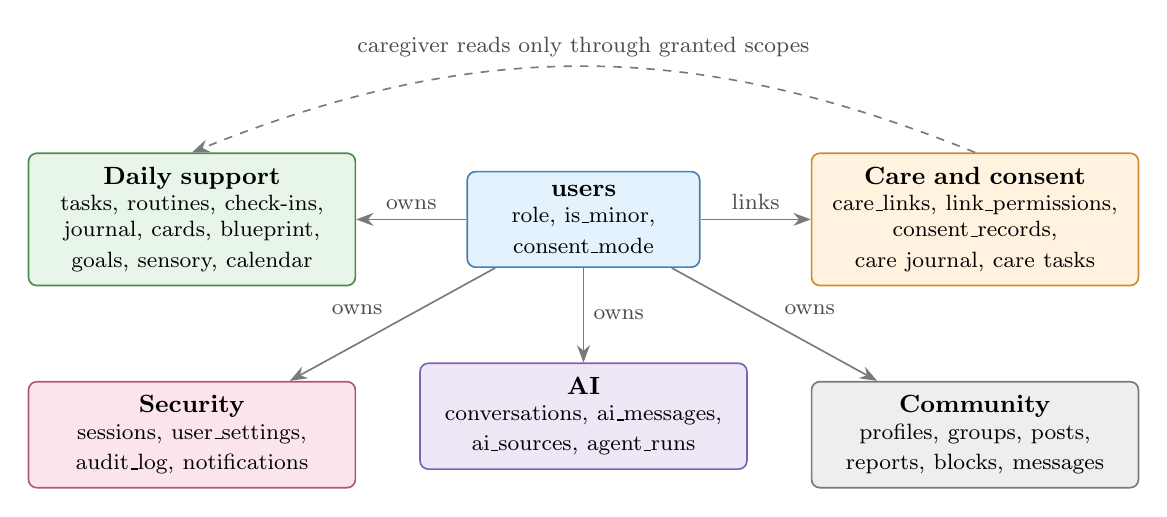
\begin{tikzpicture}[node distance=10mm and 14mm]
  \node[blue, text width=2.6cm] (u) {\textbf{users}\\ \footnotesize role, is\_minor,\\ \footnotesize consent\_mode};
  \node[green, left=of u, text width=3.8cm] (daily) {\textbf{Daily support}\\ \footnotesize tasks, routines, check-ins,\\ \footnotesize journal, cards, blueprint,\\ \footnotesize goals, sensory, calendar};
  \node[orange, right=of u, text width=3.8cm] (care) {\textbf{Care and consent}\\ \footnotesize care\_links, link\_permissions,\\ \footnotesize consent\_records,\\ \footnotesize care journal, care tasks};
  \node[lav, below=12mm of u, text width=3.8cm] (ai) {\textbf{AI}\\ \footnotesize conversations, ai\_messages,\\ \footnotesize ai\_sources, agent\_runs};
  \node[pink, below=12mm of daily, text width=3.8cm] (sec) {\textbf{Security}\\ \footnotesize sessions, user\_settings,\\ \footnotesize audit\_log, notifications};
  \node[gray, below=12mm of care, text width=3.8cm] (comm) {\textbf{Community}\\ \footnotesize profiles, groups, posts,\\ \footnotesize reports, blocks, messages};
  \draw[arr] (u) -- node[lbl, above]{owns} (daily);
  \draw[arr] (u) -- node[lbl, above]{links} (care);
  \draw[arr] (u) -- node[lbl, right]{owns} (ai);
  \draw[arr] (u) -- node[lbl, above left]{owns} (sec);
  \draw[arr] (u) -- node[lbl, above right]{owns} (comm);
  \draw[darr] (care.north) to[bend right=22] node[lbl, above]{caregiver reads only through granted scopes} (daily.north);
\end{tikzpicture}
\caption{Data model overview. Every record belongs to a user; a caregiver reads an individual's daily-support data only through granted scopes.}
\label{fig:datamodel}
\end{figure}

\begin{table}[H]
\centering
\caption{Database tables grouped by area (43 tables)}
\label{tab:tables}
\small
\begin{tabularx}{\textwidth}{@{}L{3.2cm}Y@{}}
\toprule
\textbf{Area} & \textbf{Tables}\\
\midrule
Accounts and security & users, sessions, user\_settings, audit\_log\\
Daily support & tasks, task\_steps, routines, routine\_steps, routine\_runs, checkins, journal\_entries, comm\_cards, blueprint\_sections, goals, sensory\_strategies, sensory\_diary, sensory\_kit, calendar\_events, focus\_sessions\\
Care and consent & care\_links, link\_permissions, consent\_records, support\_requests, care\_journal, care\_tasks, support\_notes, care\_contacts, wellbeing\_checkins\\
Community & community\_profiles, community\_groups, group\_members, posts, comments, post\_reactions, reports, blocks, connections, direct\_messages\\
AI and system & conversations, ai\_messages, ai\_sources, agent\_runs, notifications, schema\_migrations\\
\bottomrule
\end{tabularx}
\end{table}

\subsection{Environment}
\begin{table}[H]
\centering
\caption{Development and test environment}
\label{tab:env}
\small
\begin{tabular}{@{}ll@{}}
\toprule
\textbf{Component} & \textbf{Version / value}\\
\midrule
Python & 3.13\\
FastAPI / Pydantic & 0.165.0 / 2.13.5\\
Database & SQLite (Python standard library)\\
PyTorch (training smoke test, CPU) & 2.15.0\\
Transformers / PEFT / Accelerate / Datasets & 4.48.3 / 0.14.0 / 1.3.0 / 3.2.0\\
bitsandbytes (GPU training) & 0.50.2\\
Training GPU (planned) & NVIDIA Tesla T4, Google Colab\\
Browser testing & Playwright (headless Chromium) and axe-core\\
\bottomrule
\end{tabular}
\end{table}

% =====================================================================
\section{Web Application}\label{sec:webapp}
% =====================================================================

\subsection{Two Distinct Experiences}
Individuals and caregivers get genuinely different navigation and pages (Table~\ref{tab:experiences}).
Both share the Assistant, Community, Events \& groups, Providers \& appointments and Settings.

\begin{table}[H]
\centering
\caption{Main pages in the individual and caregiver experiences}
\label{tab:experiences}
\small
\begin{tabularx}{\textwidth}{@{}YY@{}}
\toprule
\textbf{Individual} & \textbf{Caregiver}\\
\midrule
\textbf{My Day}: energy check-in, one suggested starting task, today's tasks, coming up, routines, ``done today'' (resting counts) &
\textbf{Dashboard}: people I support, appointments, open support requests, care tasks, wellbeing prompt\\
\textbf{Tasks}: steps, \emph{Help me start} (one tiny action), \emph{What next?}, focus / body-doubling timer, postpone without penalty &
\textbf{Care journal}: context, what happened, what helped; private by default; pattern counts carry a ``not a cause'' notice\\
\textbf{Routines}: templates, step player, skip or swap steps, no streaks &
\textbf{Care calendar} and \textbf{Coordination}: care tasks, handovers, contacts (needs the \emph{coordination} scope)\\
\textbf{Check-in}: tap-only mood, energy, stress, sensory and social energy; words optional &
\textbf{People I support}: only the items the person has shared\\
\textbf{Sensory toolkit}, \textbf{Communication cards} (full screen, text-to-speech), private \textbf{Journal} &
\textbf{Support requests}: alerts from the person's \emph{I need someone} button, with replies\\
\textbf{Support Blueprint} (13 sections, per-section sharing, export), \textbf{Goals}, \textbf{Learn} &
\textbf{Learning hub}, \textbf{Wellbeing} (stress check-in, rest and delegation ideas, no guilt)\\
\bottomrule
\end{tabularx}
\end{table}

\subsection{Overwhelm Mode}
The \emph{I'm overwhelmed} button sits in the header of every page. It switches to a
low-stimulation screen with one question and six large choices (Figure~\ref{fig:overwhelm}).
Breathing exercises are offered as one option and never assumed to help. \emph{I need someone} sends a
support request only to people in the user's active circle.

\begin{figure}[H]
\centering
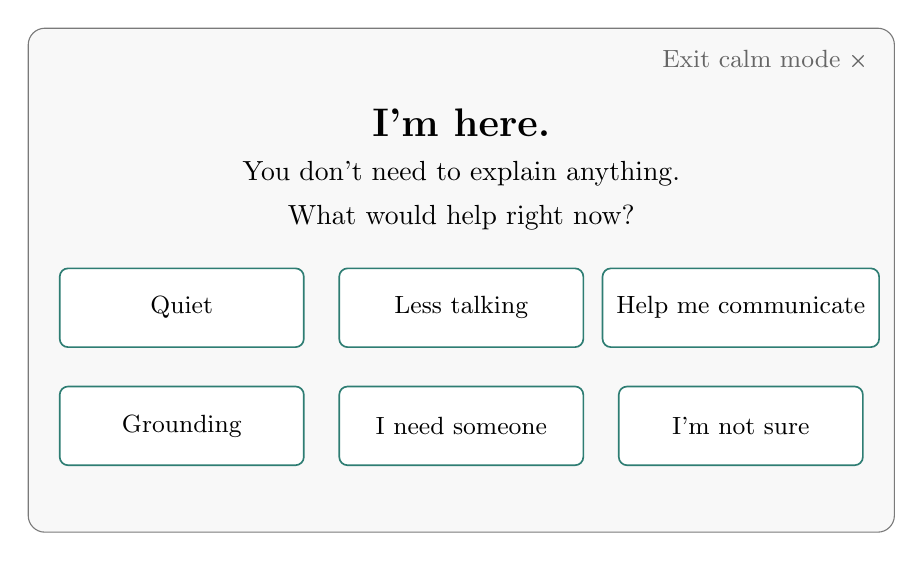
\begin{tikzpicture}
  \draw[rounded corners=6pt, fill=nbgray!40, draw=nbgrayD] (0,0) rectangle (11,6.4);
  \node[font=\small, text=black!60, anchor=north east] at (10.8,6.25) {Exit calm mode \texttimes};
  \node[font=\Large\bfseries] at (5.5,5.2) {I'm here.};
  \node[font=\normalsize] at (5.5,4.55) {You don't need to explain anything.};
  \node[font=\normalsize] at (5.5,4.0) {What would help right now?};
  \foreach \x/\y/\t in {1.95/2.85/Quiet, 5.5/2.85/Less talking, 9.05/2.85/Help me communicate,
                         1.95/1.35/Grounding, 5.5/1.35/I need someone, 9.05/1.35/I'm not sure}{
    \node[base, fill=white, draw=nbteal, minimum width=3.1cm, minimum height=1.0cm, font=\small] at (\x,\y) {\t};
  }
\end{tikzpicture}
\caption{Overwhelm mode (wireframe): one question, six choices, short sentences, no animation and an easy exit.}
\label{fig:overwhelm}
\end{figure}

\subsection{Consent Model}
A caregiver relationship does not grant access by itself. Figure~\ref{fig:consent} shows the flow,
and Listing~\ref{lst:canview} shows the single function every caregiver read passes through.

\begin{figure}[H]
\centering
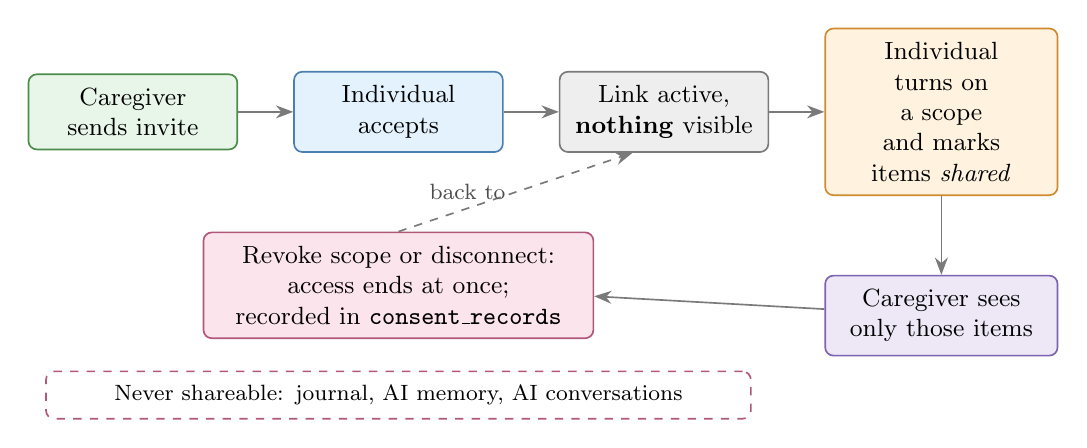
\begin{tikzpicture}[node distance=5mm and 7mm]
  \node[green, text width=2.3cm] (inv) {Caregiver\\sends invite};
  \node[blue, right=of inv, text width=2.3cm] (acc) {Individual\\accepts};
  \node[gray, right=of acc, text width=2.3cm] (none) {Link active,\\\textbf{nothing} visible};
  \node[orange, right=of none, text width=2.6cm] (grant) {Individual turns on\\a scope and marks\\items \emph{shared}};
  \node[lav, below=10mm of grant, text width=2.6cm] (view) {Caregiver sees\\only those items};
  \node[pink, below=10mm of acc, text width=4.6cm] (revoke) {Revoke scope or disconnect:\\access ends at once;\\recorded in \code{consent\_records}};
  \draw[arr] (inv) -- (acc);
  \draw[arr] (acc) -- (none);
  \draw[arr] (none) -- (grant);
  \draw[arr] (grant) -- (view);
  \draw[arr] (view) -- (revoke);
  \draw[darr] (revoke.north) -- node[lbl, left]{back to} ($(none.south)+(-0.4,0)$) ;
  \node[base, fill=white, draw=nbpinkD, dashed, below=4mm of revoke, text width=8.6cm, font=\footnotesize]
    {Never shareable: journal, AI memory, AI conversations};
\end{tikzpicture}
\caption{Consent flow between a caregiver and an individual. Each scope (blueprint, routines, calendar, goals, tasks, check-in summary, coordination) is granted separately.}
\label{fig:consent}
\end{figure}

\par\noindent\begin{minipage}{\linewidth}\begin{lstlisting}[caption={Every caregiver read is checked against the granted scopes (\code{nbapp/consent.py}).},label={lst:canview}]
SCOPES = {
    "blueprint": "Shared parts of My Support Blueprint",
    "routines": "Routines you mark as shared",
    "calendar": "Calendar events you mark as shared",
    "goals": "Goals you mark as shared",
    "tasks": "Tasks you mark as shared",
    "checkin_summary": "A weekly summary of check-ins (not the notes)",
    "coordination": "Care tasks and shared support notes about you",
}
NEVER_SHARED = ("journal", "memory", "conversations")

def can_view(db, viewer, individual_id, scope):
    """True if `viewer` may see `scope` data of `individual_id`."""
    if viewer["id"] == individual_id:
        return True
    if scope not in SCOPES:          # journal, memory, conversations never match
        return False
    link = link_between(db, individual_id, viewer["id"])   # active links only
    return bool(link) and scope in granted_scopes(db, link["id"])
\end{lstlisting}\end{minipage}\par

For under-18 users the account runs in a guardian or supported-decision consent mode rather than
assuming one universal rule.

\subsection{Accounts and Security}
Passwords are hashed with PBKDF2-SHA256 and a random per-user salt (Listing~\ref{lst:pw}). Session
tokens are random, and only their SHA-256 hash is stored, so a copied database cannot be used to sign
in. Sign-in, registration, posting and the assistant are rate-limited. Sensitive operations (sharing changes,
exports, deletion, moderation) are written to an audit log. Admin accounts can be created only from
environment variables, never by self-registration.

\par\noindent\begin{minipage}{\linewidth}\begin{lstlisting}[caption={Password hashing and constant-time verification (\code{nbapp/security.py}).},label={lst:pw}]
ITERATIONS = 310_000

def hash_password(password: str) -> str:
    salt = os.urandom(16)
    dk = hashlib.pbkdf2_hmac("sha256", password.encode(), salt, ITERATIONS)
    return "pbkdf2_sha256${}${}${}".format(ITERATIONS, base64.b64encode(salt).decode(),
                                          base64.b64encode(dk).decode())

def verify_password(password: str, stored: str) -> bool:
    try:
        algo, iters, salt_b64, dk_b64 = stored.split("$")
        if algo != "pbkdf2_sha256":
            return False
        dk = hashlib.pbkdf2_hmac("sha256", password.encode(),
                                 base64.b64decode(salt_b64), int(iters))
        return hmac.compare_digest(dk, base64.b64decode(dk_b64))
    except Exception:
        return False
\end{lstlisting}\end{minipage}\par

\subsection{Community Connect}
Community Connect has 14 starter groups, listed in Table~\ref{tab:groups}. Members join with a handle (not a real name) and
must accept the guidelines. Features include posts, replies, supportive reactions, peer connections,
private messages between connected adults, report, block, a moderator queue, and user-proposed
events that an admin reviews.

\begin{table}[H]
\centering
\caption{Starter groups and clubs in Community Connect}
\label{tab:groups}
\small
\begin{tabularx}{\textwidth}{@{}lYl@{}}
\toprule
\textbf{Group} & \textbf{Purpose} & \textbf{Audience}\\
\midrule
ADHD body-doubling corner & Plan a task, post it, check back in & Everyone\\
Autistic adults lounge & Peer space by and for autistic adults & Adults\\
Parents \& caregivers circle & Share what is working and what is hard & Caregivers\\
Sensory tips exchange & Headphones, textures, lighting, sensory-friendly places & Everyone\\
Special interests club & Share what you love & Everyone\\
Study \& work strategies & Adjustments, planning, interviews, exams & Everyone\\
Art \& making & Drawing, crafts, music, building & Everyone\\
Goa meetups (planning) & Organise low-sensory meetups & Adults\\
Hearing voices peer space & Peer support for unusual experiences; not treatment & Adults\\
Plural \& DID respectful space & For people with DID/OSDD or who are plural, and supporters & Adults\\
Games \& puzzles club & Board games, puzzles, low-pressure chat & Everyone\\
Nature walks club & Quiet walks, birdwatching, gardening & Everyone\\
Quiet social club & Parallel play, quiet coffee mornings, text-first chat & Adults\\
Carer wellbeing circle & Carers looking after themselves too & Caregivers\\
\bottomrule
\end{tabularx}
\end{table}

Automatic checks \textbf{hold content for a human moderator and never silently delete it}
(Figure~\ref{fig:moderation}, Listing~\ref{lst:mod}). Three reports also hold a post. Under-18s can
join only groups marked safe for minors, and adults cannot message them privately.

\begin{figure}[H]
\centering
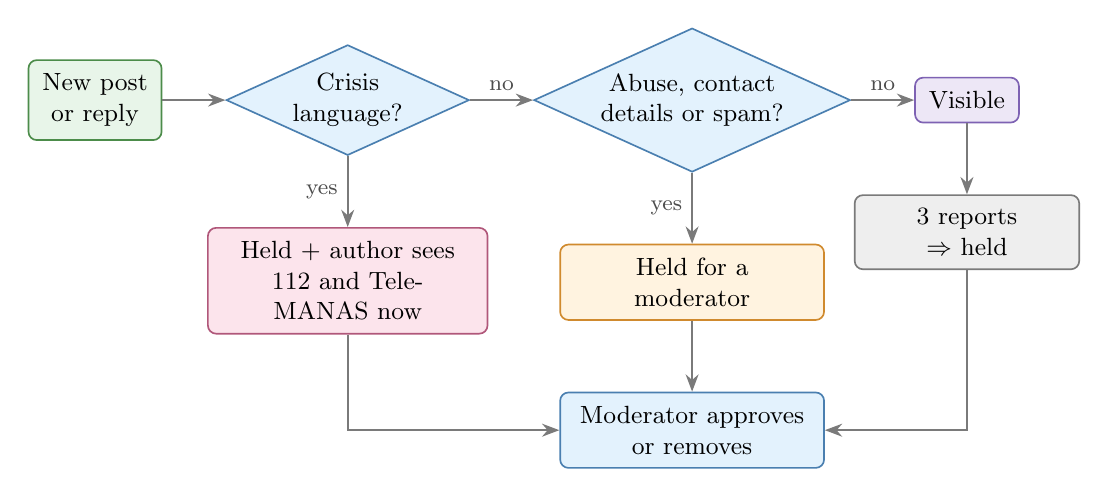
\begin{tikzpicture}[node distance=6mm and 8mm]
  \node[green] (post) {New post\\or reply};
  \node[decision, right=of post] (crisis) {Crisis\\language?};
  \node[decision, right=of crisis] (other) {Abuse, contact\\details or spam?};
  \node[lav, right=of other] (vis) {Visible};
  \node[pink, below=9mm of crisis, text width=3.2cm] (help) {Held + author sees\\112 and Tele-MANAS now};
  \node[orange, below=9mm of other, text width=3.0cm] (held) {Held for a\\moderator};
  \node[gray, below=9mm of vis, text width=2.5cm] (rep) {3 reports\\$\Rightarrow$ held};
  \node[blue, below=9mm of held, text width=3.0cm] (modq) {Moderator approves\\or removes};
  \draw[arr] (post) -- (crisis);
  \draw[arr] (crisis) -- node[lbl, above]{no} (other);
  \draw[arr] (other) -- node[lbl, above]{no} (vis);
  \draw[arr] (crisis) -- node[lbl, left]{yes} (help);
  \draw[arr] (other) -- node[lbl, left]{yes} (held);
  \draw[arr] (vis) -- (rep);
  \draw[arr] (held) -- (modq);
  \draw[arr] (help.south) |- (modq.west);
  \draw[arr] (rep.south) |- (modq.east);
\end{tikzpicture}
\caption{Community moderation. Automatic checks only ever hold content; a person makes the final decision.}
\label{fig:moderation}
\end{figure}

\par\noindent\begin{minipage}{\linewidth}\begin{lstlisting}[caption={Automatic community checks hold content; they never delete it (\code{nbapp/moderation.py}, shortened).},label={lst:mod}]
def check(text, author_is_minor=False):
    """Returns (status, reason, message_for_author)."""
    safety = classify_input(text)          # same classifier as the assistant
    if safety["category"] in ("self_harm", "emergency",
                              "psychosis_crisis", "harm_to_others"):
        return "held", "safety", CRISIS_MESSAGE      # shows 112 and Tele-MANAS 14416
    if ABUSE_RE.search(text):
        return "held", "abuse", "A moderator will review it first."
    if PHONE_RE.search(text) or EMAIL_RE.search(text) or ADDRESS_RE.search(text):
        return "held", "personal_info", "Posts with contact details are checked first."
    if SPAM_RE.search(text):
        return "held", "spam", "This looks like spam, so a moderator will review it."
    return "visible", None, None
\end{lstlisting}\end{minipage}\par

\subsection{Events, Clubs and Appointments}
The Events \& groups page lists support groups, workshops, clubs, gatherings and community
meetings. Before registering, the user sees the exact title, time, place, fee and number of
attendees. The approval is bound to a fingerprint of those details (Listing~\ref{lst:hash}), and the
registration is refused if anything changed afterwards (Figure~\ref{fig:booking}). Full events put the
user on a waitlist, and a cancellation promotes the next person.

\par\noindent\begin{minipage}{\linewidth}\begin{lstlisting}[caption={Approval is bound to a fingerprint of everything the person agreed to (\code{agent/tools/events\_db.py}, shortened).},label={lst:hash}]
def details_fingerprint(event, attendees):
    """Hash of everything the person is agreeing to."""
    payload = json.dumps([event["event_id"], event["title"], event["start_time"],
                          event["end_time"], event["location"], bool(event["is_online"]),
                          float(event["fee_amount"] or 0), event["fee_currency"],
                          int(attendees)], sort_keys=True)
    return hashlib.sha256(payload.encode()).hexdigest()[:16]

def register(self, event_id, user_id, attendees=1, approved_details_hash=None,
             explicit_approval=False):
    if explicit_approval is not True or not approved_details_hash:
        return {"success": False, "message": "Explicit approval is required."}
    current = details_fingerprint(event, attendees)
    if current != approved_details_hash:
        return {"success": False, "approval_stale": True,
                "message": "The event details changed after you approved."}
    ...  # confirm if seats remain, otherwise waitlist; return a confirmation code
\end{lstlisting}\end{minipage}\par

\begin{figure}[H]
\centering
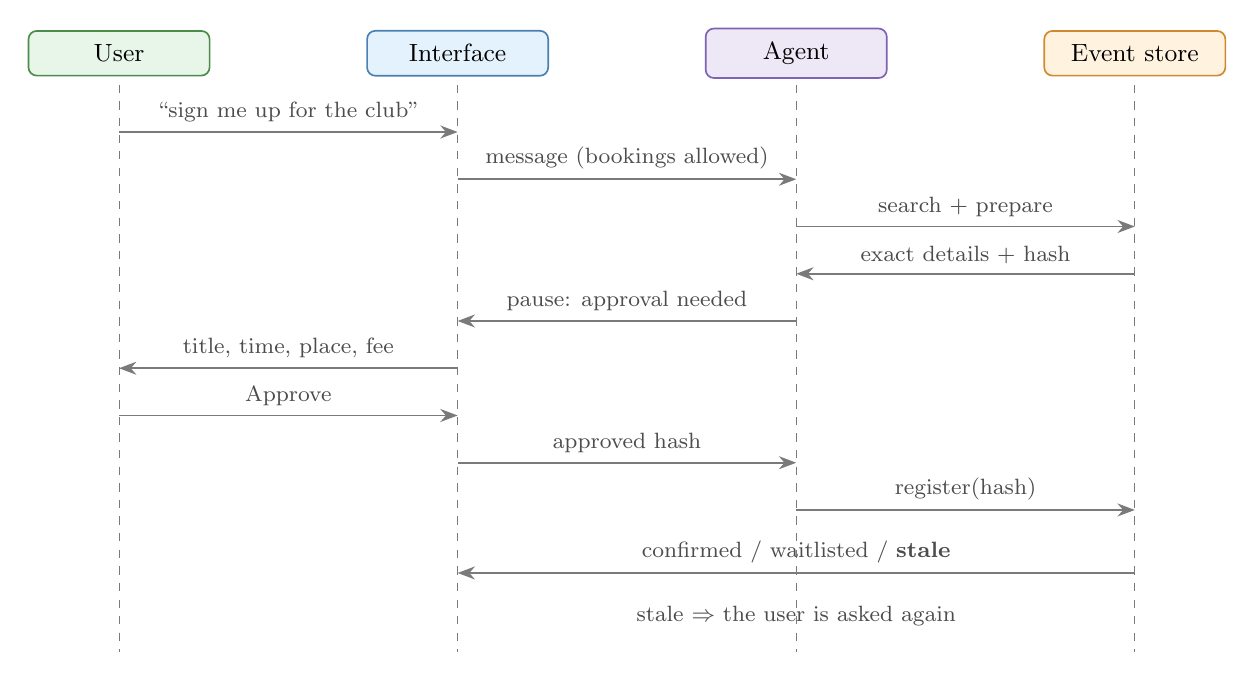
\begin{tikzpicture}[font=\small]
  \foreach \x/\n/\c in {0/User/green, 4.3/Interface/blue, 8.6/Agent/lav, 12.9/Event store/orange}{
    \node[\c, minimum width=2.3cm] (h\n) at (\x,0) {\n};
    \draw[nbgrayD, dashed] (\x,-0.4) -- (\x,-7.6);
  }
  \newcommand{\msg}[4]{\draw[arr] (#1,#3) -- node[lbl, above]{#4} (#2,#3);}
  \msg{0}{4.3}{-1.0}{``sign me up for the club''}
  \msg{4.3}{8.6}{-1.6}{message (bookings allowed)}
  \msg{8.6}{12.9}{-2.2}{search + prepare}
  \msg{12.9}{8.6}{-2.8}{exact details + hash}
  \msg{8.6}{4.3}{-3.4}{pause: approval needed}
  \msg{4.3}{0}{-4.0}{title, time, place, fee}
  \msg{0}{4.3}{-4.6}{Approve}
  \msg{4.3}{8.6}{-5.2}{approved hash}
  \msg{8.6}{12.9}{-5.8}{register(hash)}
  \msg{12.9}{4.3}{-6.6}{confirmed / waitlisted / \textbf{stale}}
  \node[lbl] at (8.6,-7.15) {stale $\Rightarrow$ the user is asked again};
\end{tikzpicture}
\caption{Booking an event through the assistant. Nothing is registered until the user approves the exact details, and a changed detail makes the approval stale.}
\label{fig:booking}
\end{figure}

Appointments with providers follow the same pattern. Only providers verified by an admin are listed.
Requests move from \emph{requested} to \emph{pending approval} to \emph{confirmed} or
\emph{cancelled}, and nothing is shown as booked unless the database confirms it. Sample events are
visibly labelled \emph{Demo listing --- not a real event}.

\subsection{Accessibility and Design}
The interface uses a calm palette of warm neutrals, soft teal, lavender and sage, with semantic
HTML, visible focus rings and live regions for chat updates. Settings offer dark mode, high contrast,
low-stimulation mode, reduced motion, a dyslexia-friendly font, adjustable text size, short, detailed
or simple-language replies, text-to-speech, speech-to-text (in supporting browsers), quiet hours and
per-category notification switches. Notifications use no guilt-based wording and there are no streaks.

% =====================================================================
\section{AI Assistant and Deep Agent}\label{sec:agent}
% =====================================================================

\subsection{One Assistant, Two Engines}
A single endpoint, \code{POST /api/assistant/message}, joins the chat LLM and the research agent.
In \emph{Auto} mode it decides which one to use (Figure~\ref{fig:routing}, Listing~\ref{lst:route});
the user can also choose Chat or Research \& actions directly.

\begin{figure}[H]
\centering
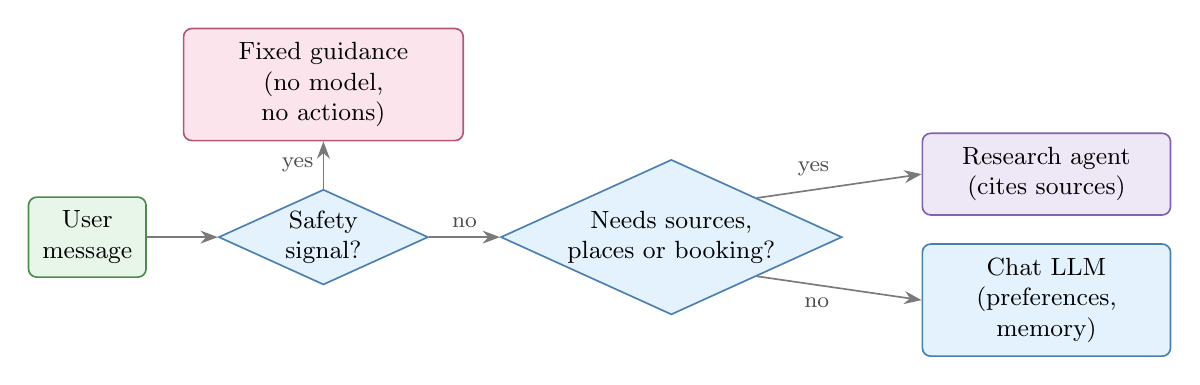
\begin{tikzpicture}[node distance=6mm and 9mm]
  \node[green] (m) {User\\message};
  \node[decision, right=of m] (s) {Safety\\signal?};
  \node[pink, above=6mm of s, text width=3.2cm] (fix) {Fixed guidance\\(no model, no actions)};
  \node[decision, right=of s] (r) {Needs sources,\\places or booking?};
  \node[lav, right=10mm of r, yshift=8mm, text width=2.8cm] (agent) {Research agent\\(cites sources)};
  \node[blue, right=10mm of r, yshift=-8mm, text width=2.8cm] (chat) {Chat LLM\\(preferences, memory)};
  \draw[arr] (m) -- (s);
  \draw[arr] (s) -- node[lbl, left]{yes} (fix);
  \draw[arr] (s) -- node[lbl, above]{no} (r);
  \draw[arr] (r.north east) -- node[lbl, above left]{yes} (agent.west);
  \draw[arr] (r.south east) -- node[lbl, below left]{no} (chat.west);
\end{tikzpicture}
\caption{Assistant routing. Safety runs before either engine.}
\label{fig:routing}
\end{figure}

\par\noindent\begin{minipage}{\linewidth}\begin{lstlisting}[caption={Auto-routing between chat and the agent (\code{nbapp/assistant.py}, shortened).},label={lst:route}]
AGENT_RE = re.compile(r"\b(research|search (?:for|the web)|look up|sources?|citations?|"
    r"evidence|latest|news|near me|nearby|therapists?|clinics?|providers?|"
    r"organi[sz]ations?|support groups?|workshops?|clubs?|gatherings?|events?|"
    r"book|booking|register|sign me up|appointments?|schemes?|helplines?)\b", re.I)
CHAT_FIRST_RE = re.compile(r"^(?:how do i|how can i|help me (?:write|draft|plan|start|"
    r"understand)|can you explain|what is|what are|why do|i feel|i'm|im )", re.I)

def decide_mode(message: str) -> str:
    text = message.strip()
    if CHAT_FIRST_RE.search(text) and not re.search(
            r"\b(near me|sources?|research|book|register|sign me up)\b", text, re.I):
        return "chat"
    return "agent" if AGENT_RE.search(text) else "chat"
\end{lstlisting}\end{minipage}\par

Chat replies use the person's settings (short, detailed or simple language) and, if memory is
switched on, their saved memories. Each reply states which context it used. A caregiver's assistant can
only use what the individual has shared. The system prompt tells the model to offer one small first
step for task help, never to claim it has acted, and to be soft but plain that 112 must be called
in serious situations.

\subsection{The Agent Loop}
Figure~\ref{fig:loop} shows how an agent run proceeds from plan to verified answer.

\begin{figure}[H]
\centering
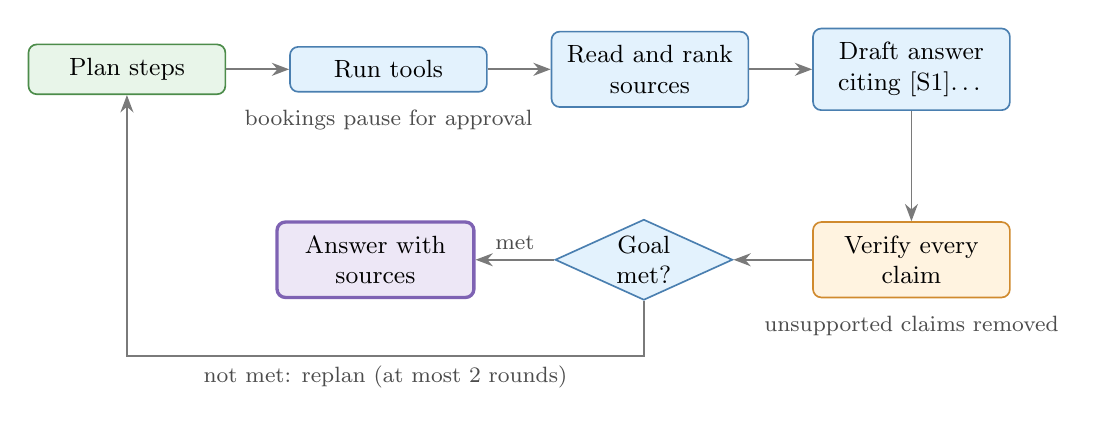
\begin{tikzpicture}[node distance=6mm and 8mm]
  \node[green, minimum width=2.5cm] (plan) {Plan steps};
  \node[blue, right=of plan, minimum width=2.5cm] (tools) {Run tools};
  \node[blue, right=of tools, minimum width=2.5cm] (read) {Read and rank\\sources};
  \node[blue, right=of read, minimum width=2.5cm] (draft) {Draft answer\\citing [S1]\ldots};
  \node[orange, below=14mm of draft, minimum width=2.5cm] (ver) {Verify every\\claim};
  \node[decision, left=10mm of ver] (goal) {Goal\\met?};
  \node[lav, left=10mm of goal, minimum width=2.5cm, line width=1.2pt] (ans) {Answer with\\sources};
  \node[lbl, below=1mm of tools] {bookings pause for approval};
  \node[lbl, below=1mm of ver] {unsupported claims removed};
  \draw[arr] (plan) -- (tools);
  \draw[arr] (tools) -- (read);
  \draw[arr] (read) -- (draft);
  \draw[arr] (draft) -- (ver);
  \draw[arr] (ver) -- (goal);
  \draw[arr] (goal) -- node[lbl, above]{met} (ans);
  \draw[arr] (goal.south) -- ++(0,-0.7) -| node[lbl, below, pos=0.25]{not met: replan (at most 2 rounds)} (plan.south);
\end{tikzpicture}
\caption{The agent loop: plan, execute, observe, draft, verify, check the goal, and replan if needed.}
\label{fig:loop}
\end{figure}

\begin{enumerate}
  \item \textbf{Plan.} The LLM proposes tasks. The plan is validated before anything runs: unknown tools are removed, arguments are cleaned, the signed-in user is forced into every call, and a search step is added if missing. A fixed fallback plan is used if the planner fails.
  \item \textbf{Execute.} Tools run with retries on transient errors. A tool that reports failure is recorded as a failure, never as a success; the original code had this bug.
  \item \textbf{Read and rank.} The top pages are read and evidence is ranked and numbered S1, S2,~\ldots
  \item \textbf{Draft.} The answer must cite the numbered sources.
  \item \textbf{Verify.} A deterministic check runs first (Listing~\ref{lst:verify}). An LLM verifier may then tighten the result but never loosen it. Unsupported sentences are redacted, and a redacted run can be marked at most \emph{partial}.
  \item \textbf{Goal check.} An LLM judge compares the answer with the user's criteria. If the judge itself fails, the run is never marked \emph{complete}. If criteria are unmet, the agent replans, at most twice.
\end{enumerate}

\par\noindent\begin{minipage}{\linewidth}\begin{lstlisting}[caption={Deterministic grounding check: specific facts must appear in the retrieved evidence (\code{agent/research/verification.py}, shortened).},label={lst:verify}]
def deterministic_check(answer, ranked, goal_text=""):
    evidence = ranked.get("evidence", [])
    corpus = "\n".join(" ".join([e.get("title", ""), e.get("content", ""),
                                 e.get("page_content", ""), e.get("url", "")])
                       for e in evidence)
    critical, unsupported = [], []
    for url in URL_RE.findall(answer):
        if _norm_url(url) not in evidence_urls:
            critical.append({"type": "unsupported_url", "value": url})
    for phone in PHONE_RE.findall(answer):
        digits = _norm_digits(phone)
        if len(digits) >= 9 and digits not in corpus_digits and digits not in ALLOWED_DIGITS:
            critical.append({"type": "unsupported_phone", "value": phone.strip()})
    for price in PRICE_RE.findall(answer):
        if _norm_digits(price) not in corpus_digits:
            critical.append({"type": "unsupported_price", "value": price})
    for entity in candidate_entities(answer):        # e.g. "Sunrise Autism Trust"
        if is_organisation(entity) and entity.lower() not in corpus.lower():
            unsupported.append({"type": "unsupported_entity", "value": entity})
    cited = {int(n) for n in CITATION_RE.findall(answer)}
    if any(n < 1 or n > len(evidence) for n in cited):
        critical.append({"type": "invalid_citation"})
    passed = not critical and not unsupported and bool(evidence) and bool(cited)
    ...
\end{lstlisting}\end{minipage}\par

\subsection{Approvals}
When the plan reaches a tool marked \emph{approval required}, such as event registration or an appointment
request, the run pauses and the interface shows a plain summary of the exact action. Bookings also
require the user to tick \emph{Allow bookings} in the message box, so a research question can never
book by accident. The approval carries the details hash (Listing~\ref{lst:hash}), so the tool refuses
any call whose details no longer match.

\subsection{Language Models and Complete Replies}
All model calls go through one gateway with a provider registry and fallback. Hosted models
sometimes stop at the token limit and leave a reply half-finished. The gateway detects this and asks the same
provider to continue, up to twice (Listing~\ref{lst:continue}). During a side-by-side comparison
fallback is switched off, so a failing model shows an error instead of another model's answer.

\par\noindent\begin{minipage}{\linewidth}\begin{lstlisting}[caption={Automatic continuation of replies cut off by the token limit (\code{agent/llm/gateway.py}).},label={lst:continue}]
auto_continue = kwargs.pop("auto_continue", 2)
response = self._generate_once(primary_name, messages, system_prompt,
                               temperature, max_tokens, **kwargs)
parts, rounds = [response.text], 0
while response.metadata.get("truncated") and rounds < auto_continue:
    rounds += 1
    follow = list(messages) + [
        {"role": "assistant", "content": "".join(parts)},
        {"role": "user", "content": "Continue exactly where you stopped. "
                                    "Do not repeat anything already written."}]
    try:
        response = self._generate_once(response.provider, follow, system_prompt,
                                       temperature, max_tokens, **kwargs)
    except Exception:
        break
    parts.append(response.text)
if rounds:
    response.text = "".join(parts)
    response.metadata["continued"] = rounds
\end{lstlisting}\end{minipage}\par

\subsection{Serving Base, SFT and SFT+ORPO Together}
The three NeuroBridge models share one copy of Qwen2.5-1.5B in memory. The SFT and ORPO
adapters are loaded by name and switched per request, and the base model is used by disabling the
adapters (Figure~\ref{fig:adapters}, Listing~\ref{lst:adapters}). All three therefore fit on a single T4
GPU, and a \emph{Compare} view sends one message to all three.

\begin{figure}[H]
\centering
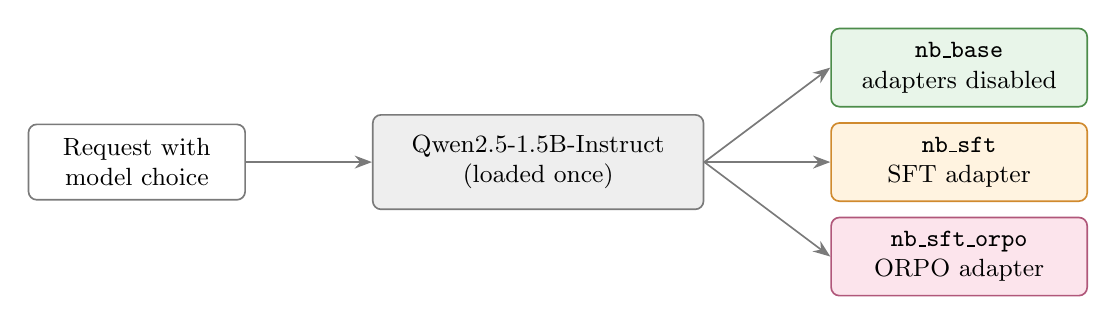
\begin{tikzpicture}[node distance=5mm and 10mm]
  \node[gray, minimum width=4.2cm, minimum height=1.2cm] (base) {Qwen2.5-1.5B-Instruct\\(loaded once)};
  \node[base, fill=white, draw=nbgrayD, left=16mm of base, text width=2.4cm] (req) {Request with\\model choice};
  \node[green, right=16mm of base, yshift=12mm, text width=2.9cm] (b) {\code{nb\_base}\\adapters disabled};
  \node[orange, right=16mm of base, text width=2.9cm] (s) {\code{nb\_sft}\\SFT adapter};
  \node[pink, right=16mm of base, yshift=-12mm, text width=2.9cm] (o) {\code{nb\_sft\_orpo}\\ORPO adapter};
  \draw[arr] (req) -- (base);
  \draw[arr] (base.east) -- (b.west);
  \draw[arr] (base.east) -- (s.west);
  \draw[arr] (base.east) -- (o.west);
\end{tikzpicture}
\caption{Multi-adapter serving: one base model in memory, three selectable configurations.}
\label{fig:adapters}
\end{figure}

\par\noindent\begin{minipage}{\linewidth}\begin{lstlisting}[caption={Switching adapters per request (\code{agent/llm/hf\_provider.py}, shortened).},label={lst:adapters}]
def generate(self, adapter, msgs, max_new_tokens, temperature):
    with self.lock:                       # one request at a time on the shared model
        self.load()
        ids = self.tok.apply_chat_template(msgs, add_generation_prompt=True,
                                           return_tensors="pt").to(self.model.device)
        if adapter:
            if adapter not in self.adapters:
                raise RuntimeError(f"Adapter not loaded: {adapter}")
            self.model.set_adapter(adapter)
            ctx = contextlib.nullcontext()
        else:                             # base model: switch adapters off
            ctx = self.model.disable_adapter() if self.adapters else contextlib.nullcontext()
        with torch.no_grad(), ctx:
            out = self.model.generate(ids, attention_mask=torch.ones_like(ids), **gen)
        new = out[0][ids.shape[-1]:]
        return self.tok.decode(new, skip_special_tokens=True).strip()
\end{lstlisting}\end{minipage}\par

% =====================================================================
\section{Safety Layer}\label{sec:safety}
% =====================================================================

\subsection{Design}
The most dangerous messages never reach a language model. They get fixed, sourced text that cannot
be cut off or invented. Other sensitive messages are answered by the model with a policy note added to
the prompt, and a filter checks the output (Figure~\ref{fig:safety}).

\begin{figure}[H]
\centering
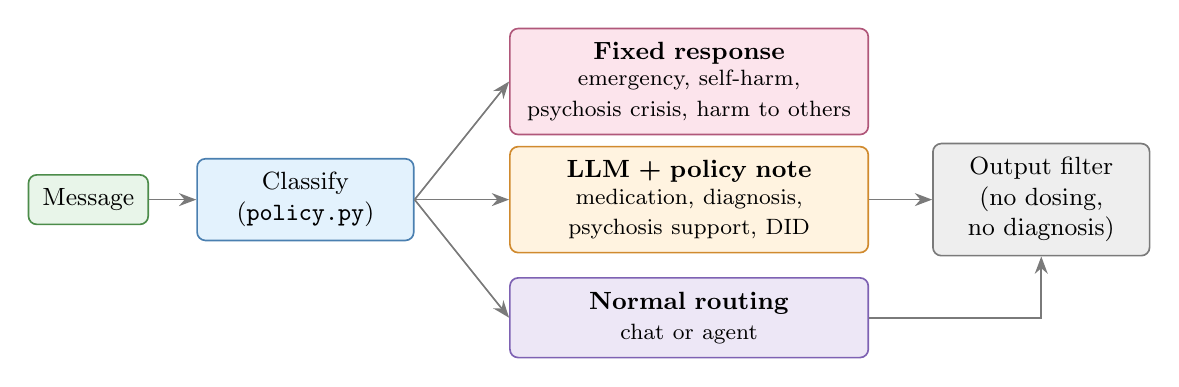
\begin{tikzpicture}[node distance=6mm and 6mm]
  \node[green] (in) {Message};
  \node[blue, right=of in, text width=2.4cm] (cls) {Classify\\(\code{policy.py})};
  \node[pink, right=12mm of cls, yshift=15mm, text width=4.2cm] (fixed) {\textbf{Fixed response}\\ \footnotesize emergency, self-harm,\\ \footnotesize psychosis crisis, harm to others};
  \node[orange, right=12mm of cls, text width=4.2cm] (note) {\textbf{LLM + policy note}\\ \footnotesize medication, diagnosis,\\ \footnotesize psychosis support, DID};
  \node[lav, right=12mm of cls, yshift=-15mm, text width=4.2cm] (normal) {\textbf{Normal routing}\\ \footnotesize chat or agent};
  \node[gray, right=8mm of note, text width=2.4cm] (filter) {Output filter\\(no dosing,\\no diagnosis)};
  \draw[arr] (in) -- (cls);
  \draw[arr] (cls.east) -- (fixed.west);
  \draw[arr] (cls.east) -- (note.west);
  \draw[arr] (cls.east) -- (normal.west);
  \draw[arr] (note) -- (filter);
  \draw[arr] (normal.east) -| (filter.south);
\end{tikzpicture}
\caption{Safety triage. Only the lower two paths involve a language model.}
\label{fig:safety}
\end{figure}

\begin{table}[H]
\centering
\caption{Safety categories and responses}
\label{tab:safety}
\small
\begin{tabularx}{\textwidth}{@{}L{3.1cm}YL{5.3cm}@{}}
\toprule
\textbf{Category} & \textbf{Example trigger} & \textbf{Response}\\
\midrule
Emergency (first aid) & ``my son is choking'', ``she's not breathing'', seizure, stroke signs, heavy bleeding, overdose, head injury & Fixed guide: calm opening, ``call 112 now'', numbered steps, what not to do\\
Self-harm & intent or plan to hurt oneself & Fixed crisis reply: 112, Tele-MANAS 14416 / 1-800-891-4416\\
Psychosis crisis & voices telling the person to harm someone & Fixed reply: stay safe, call 112, do not argue with the voices\\
Harm to others & stated intent to hurt someone & Fixed reply with 112\\
Medication / diagnosis & ``should I stop her meds?'', ``does he have autism?'' & LLM with policy note: no dosing or diagnosis; suggest a professional\\
Psychosis support / DID & hearing voices, switching, alters & LLM with note: calm, respect each part's name, neither agree nor argue about unusual beliefs\\
\bottomrule
\end{tabularx}
\end{table}

\subsection{First-Aid Guidance}
Eight fixed guides cover choking (adult and baby), CPR, seizure, stroke, bleeding, poisoning and
head injury. They were written from NHS, CDC, Resuscitation Council UK, British Red Cross and St John
Ambulance guidance~\cite{nhs,cdc,resus,redcross}. Each guide opens with a calming line (``I'm here
with you. Take one slow breath --- you're doing the right thing by acting now.''), then states firmly that
the person must call 112, followed by numbered steps and a list of what not to do.

Detection uses present-tense patterns (Listing~\ref{lst:detect}), so ``what foods are choking
hazards for toddlers?'' is answered as an ordinary question rather than treated as an emergency.

\par\noindent\begin{minipage}{\linewidth}\begin{lstlisting}[caption={Present-tense emergency detection (\code{agent/safety/first\_aid.py}, excerpt).},label={lst:detect}]
DETECT = [
    ("choking_baby", r"\b(baby|infant|newborn)\b.{0,40}\b(is choking|choking on|"
                     r"choking right now|can'?t breathe|isn'?t breathing|not breathing)"),
    ("choking", r"\b(is|are|'s|keeps|started|start) choking\b(?! (?:hazard|risk))"
                r"|\bchoking (right )?now\b|\bchoking on\b"
                r"|something (is )?stuck in (his|her|their|my) throat"),
    ("cpr", r"\b(not breathing|stopped breathing|isn'?t breathing|no pulse|"
            r"unresponsive|unconscious|won'?t wake up|collapsed)\b"),
    ("seizure", r"\b(is|'s|are) (having|in) an? (seizure|fit)\b"
                r"|\bseizure (won'?t|isn'?t|is not|hasn'?t) stop"),
    # ... stroke, bleeding, poisoning, head_injury
]

def render(key):
    g = GUIDES[key]
    lines = [CALM_OPEN, "", f"**{g['stance']}**", "",
             f"**What to do - {g['title'].lower()}:**"]
    lines += [f"{i}. {s}" for i, s in enumerate(g["steps"], 1)]
    if g["avoid"]:
        lines += ["", "**Please don't:**"] + [f"- {a}" for a in g["avoid"]]
    ...
\end{lstlisting}\end{minipage}\par

\subsection{Limits of the Safety Layer}
Detection is keyword- and pattern-based. It will miss some paraphrased or non-English emergencies and
produce some false positives; only a few Hindi terms are covered. The fixed texts have not yet been
reviewed by a certified first-aid trainer or a clinician.

% =====================================================================
\section{Dataset Review and LLM Pipeline}\label{sec:llm}
% =====================================================================

\subsection{Dataset Audit}
The original training notebook was replayed to recover its data files, which were then measured
(Table~\ref{tab:audit}).

\begin{table}[H]
\centering
\caption{Audit of the inherited and added training data}
\label{tab:audit}
\small
\begin{tabularx}{\textwidth}{@{}L{2.9cm}L{2.2cm}YL{3.3cm}@{}}
\toprule
\textbf{Dataset} & \textbf{Size} & \textbf{Finding} & \textbf{Decision}\\
\midrule
Seed set & 39 records, 12 domains & Hand-written; review marked 31 keep, 8 revise & Kept verbatim; core data\\
Long-form v2 & 36 records & Good content, but about 2,171 characters each versus about 377 in the seed set & Kept, length flagged\\
Templated SFT & 12,000 rows & 768 unique instructions; responses built from 164 distinct lines; 25\% contain a leaked instruction; 96\% a broken sentence splice & Repaired; opt-in only, labelled\\
ORPO pairs & 1,000 pairs & Only 8 distinct rejected answers, all strawmen & Quarantined\\
Neurodivergent mental-health additions & 19 records & DID 5, psychosis 6, autism/ADHD/sensory 5, emergency 3; synthetic & Labelled synthetic; clinician review pending\\
\bottomrule
\end{tabularx}
\end{table}

An earlier SFT run in the notebook on the 12,000 rows reached a training loss of 0.23 and reproduced the leaked
instruction in its own outputs. That is memorisation, not learning.

\subsection{Curation Pipeline}
\begin{figure}[H]
\centering
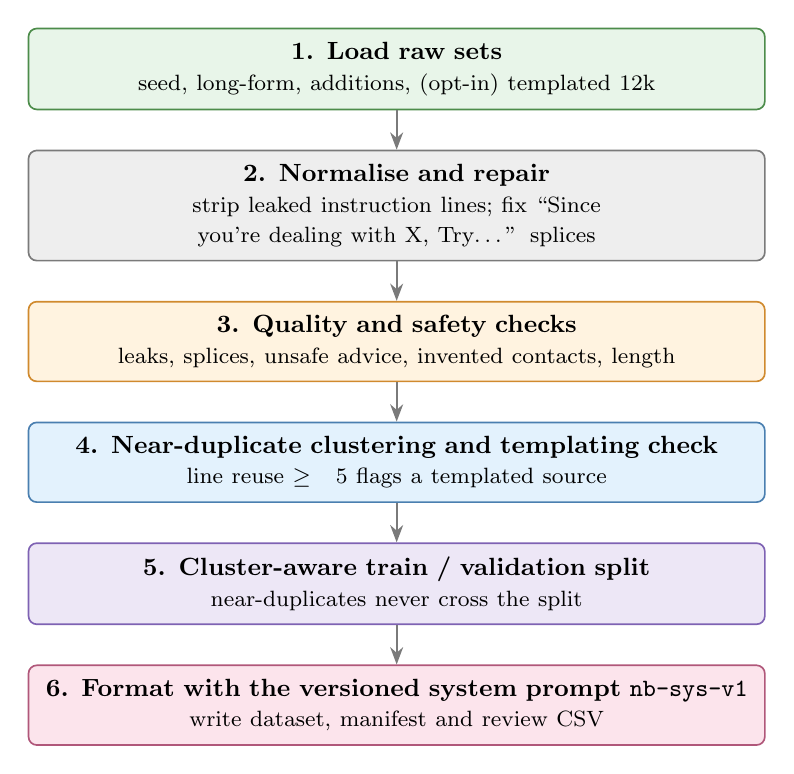
\begin{tikzpicture}[node distance=5mm]
  \node[green, text width=9cm] (s1) {\textbf{1. Load raw sets}\\ \footnotesize seed, long-form, additions, (opt-in) templated 12k};
  \node[gray, below=of s1, text width=9cm] (s2) {\textbf{2. Normalise and repair}\\ \footnotesize strip leaked instruction lines; fix ``Since you're dealing with X, Try\ldots'' splices};
  \node[orange, below=of s2, text width=9cm] (s3) {\textbf{3. Quality and safety checks}\\ \footnotesize leaks, splices, unsafe advice, invented contacts, length};
  \node[blue, below=of s3, text width=9cm] (s4) {\textbf{4. Near-duplicate clustering and templating check}\\ \footnotesize line reuse $\geq 5$ flags a templated source};
  \node[lav, below=of s4, text width=9cm] (s5) {\textbf{5. Cluster-aware train / validation split}\\ \footnotesize near-duplicates never cross the split};
  \node[pink, below=of s5, text width=9cm] (s6) {\textbf{6. Format with the versioned system prompt \code{nb-sys-v1}}\\ \footnotesize write dataset, manifest and review CSV};
  \foreach \a/\b in {s1/s2,s2/s3,s3/s4,s4/s5,s5/s6} \draw[arr] (\a) -- (\b);
\end{tikzpicture}
\caption{Dataset curation pipeline (standard-library Python, driven by versioned config files).}
\label{fig:curation}
\end{figure}

Templated sources are detected by how often each distinct response line is reused
(Listing~\ref{lst:templ}). The 12,000-row set reuses each line about 23.6 times, and still about 21.5 times
after repair.

\par\noindent\begin{minipage}{\linewidth}\begin{lstlisting}[caption={Detecting templated data by line reuse (\code{nbllm/quality.py}, shortened).},label={lst:templ}]
def templated_source_check(records, cfg, accepted=None):
    """A source whose responses are built from very few distinct lines is a template dump."""
    for name, rows in by_set.items():            # unique prompts per source
        occurrences = [l.strip() for r in rows for l in r.response.split("\n") if l.strip()]
        lines = set(occurrences)
        reuse = len(occurrences) / max(1, len(lines))   # times each line is reused
        templated = len(rows) >= 50 and reuse >= cfg.get("template_line_reuse", 5)
        if templated:
            sev = "warn" if name in accepted else "error"   # opt-in needs a reason
            for r in rows:
                r.flag("templated_source", sev,
                       f"{len(lines)} distinct lines / {len(rows)} unique prompts")
\end{lstlisting}\end{minipage}\par

\begin{table}[H]
\centering
\caption{Dataset builds produced by the pipeline}
\label{tab:builds}
\small
\begin{tabular}{@{}lrrr@{}}
\toprule
\textbf{Build} & \textbf{Records} & \textbf{Train} & \textbf{Validation}\\
\midrule
\code{dataset\_v1} (seed + long-form) & 75 & 64 & 11\\
\code{dataset\_v2\_curated} (+ additions) & 94 & 80 & 14\\
\code{dataset\_v2\_with\_12k} (+ repaired templated) & 862 & 776 & 86\\
\midrule
Safety probes (never trained on) & 32 & -- & --\\
\bottomrule
\end{tabular}
\end{table}

\subsection{Training and Evaluation Pipeline}
\begin{figure}[H]
\centering
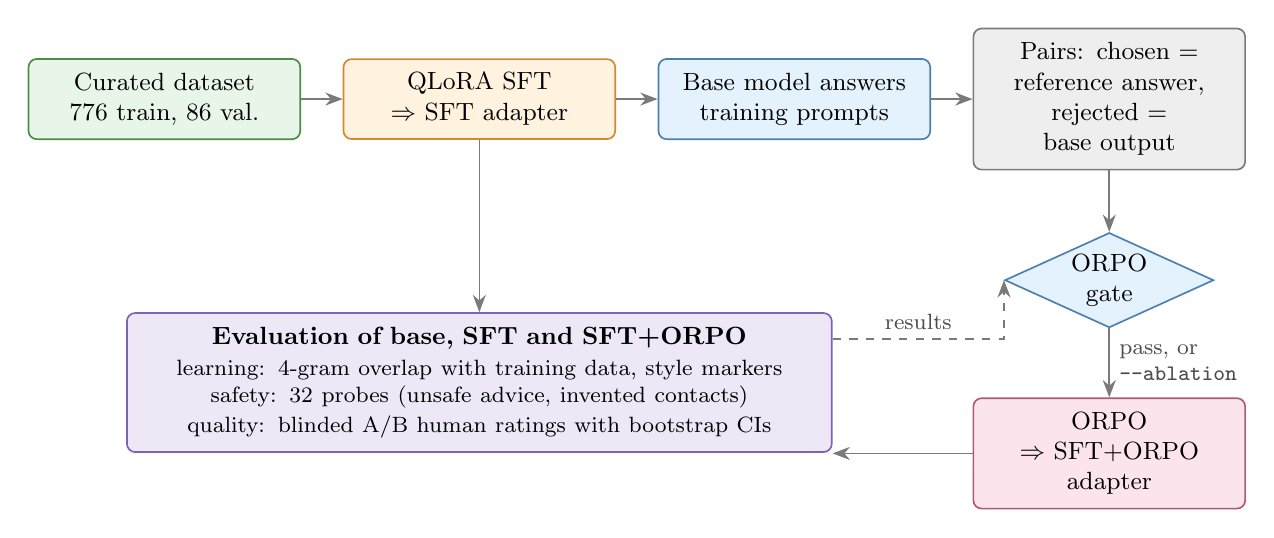
\begin{tikzpicture}
  \node[green, text width=3.1cm] (data) at (0,0) {Curated dataset\\776 train, 86 val.};
  \node[orange, text width=3.1cm] (sft) at (4,0) {QLoRA SFT\\$\Rightarrow$ SFT adapter};
  \node[blue, text width=3.1cm] (gen) at (8,0) {Base model answers\\training prompts};
  \node[gray, text width=3.1cm] (pairs) at (12,0) {Pairs: chosen =\\reference answer,\\rejected = base output};
  \node[decision] (gate) at (12,-2.3) {ORPO\\gate};
  \node[pink, text width=3.1cm] (orpo) at (12,-4.5) {ORPO\\$\Rightarrow$ SFT+ORPO adapter};
  \node[lav, text width=8.6cm] (eval) at (4,-3.6) {\textbf{Evaluation of base, SFT and SFT+ORPO}\\[2pt]
     \footnotesize learning: 4-gram overlap with training data, style markers\\
     \footnotesize safety: 32 probes (unsafe advice, invented contacts)\\
     \footnotesize quality: blinded A/B human ratings with bootstrap CIs};
  \draw[arr] (data) -- (sft);
  \draw[arr] (sft) -- (gen);
  \draw[arr] (gen) -- (pairs);
  \draw[arr] (pairs) -- (gate);
  \draw[arr] (gate) -- node[lbl, right, align=left]{pass, or\\\code{-{}-ablation}} (orpo);
  \draw[arr] (sft.south) -- (sft.south |- eval.north);
  \draw[arr] (orpo.west) -- (orpo.west -| eval.east);
  \draw[darr] (eval.east) ++(0,0.55) -| node[lbl, above, pos=0.25]{results} (gate.west);
\end{tikzpicture}
\caption{Training and evaluation pipeline. ORPO runs normally only if the gate passes; otherwise it can run only as a labelled ablation.}
\label{fig:trainpipe}
\end{figure}

\subsection{Recorded Training Configuration}
\begin{table}[H]
\centering
\caption{SFT and ORPO settings (from the config files)}
\label{tab:traincfg}
\small
\begin{tabular}{@{}lll@{}}
\toprule
\textbf{Parameter} & \textbf{SFT (\code{sft\_v2\_12k})} & \textbf{ORPO (\code{sft\_orpo\_v1})}\\
\midrule
Base model & Qwen2.5-1.5B-Instruct & starts from the SFT adapter\\
Quantization & 4-bit NF4, double quant & same\\
Compute dtype & FP16 on T4 (BF16 if supported) & same\\
LoRA rank / alpha / dropout & 16 / 32 / 0.05 & inherited\\
Target modules & q, k, v, o, gate, up, down & inherited\\
Epochs & 2 & 1\\
Batch size / grad. accumulation & 2 / 4 & 1 / 8\\
Learning rate / schedule & $1\times10^{-4}$, cosine & $1\times10^{-5}$, cosine\\
Optimizer & paged AdamW 8-bit & paged AdamW 8-bit\\
Max length & 1024 tokens & 1024 tokens\\
Loss & response-only cross-entropy & SFT + $\lambda \cdot$ odds-ratio, $\lambda=0.1$\\
Seed & 42 & 42\\
\bottomrule
\end{tabular}
\end{table}

\subsection{ORPO Implementation}
ORPO was implemented directly on the Transformers \code{Trainer} with PEFT adapters~\cite{hftransformers} (Listing~\ref{lst:orpo}) so that the
library versions already pinned for SFT did not have to change.

\par\noindent\begin{minipage}{\linewidth}\begin{lstlisting}[caption={ORPO loss as implemented (\code{nbllm/train\_orpo.py}).},label={lst:orpo}]
def orpo_loss(chosen_logps, rejected_logps, chosen_nll, lam):
    """Returns (loss, log_odds_ratio, l_or). logps are length-normalised (<= 0)."""
    eps = 1e-6
    log_odds = (chosen_logps - rejected_logps) - (
        torch.log1p(-torch.exp(chosen_logps).clamp(max=1 - eps))
        - torch.log1p(-torch.exp(rejected_logps).clamp(max=1 - eps)))
    l_or = -F.logsigmoid(log_odds)
    return chosen_nll + lam * l_or.mean(), log_odds, l_or

class ORPOTrainer(Trainer):
    lam = 0.1
    def compute_loss(self, model, inputs, return_outputs=False, num_items_in_batch=None):
        c = model(input_ids=inputs["chosen_input_ids"],
                  attention_mask=inputs["chosen_attention_mask"],
                  labels=inputs["chosen_labels"])
        r = model(input_ids=inputs["rejected_input_ids"],
                  attention_mask=inputs["rejected_attention_mask"])
        c_lp = sequence_logps(c.logits, inputs["chosen_labels"])
        r_lp = sequence_logps(r.logits, inputs["rejected_labels"])
        loss, log_odds, l_or = orpo_loss(c_lp, r_lp, c.loss, self.lam)
        return (loss, c) if return_outputs else loss
\end{lstlisting}\end{minipage}\par

\subsection{The ORPO Gate}
The project brief said ORPO must not run automatically. The gate (Table~\ref{tab:gate}) therefore checks
the evidence first. If any check fails, ORPO can only run with \code{-{}-ablation}. That run writes an
\code{ABLATION\_NOTICE.md}, and the label follows the model into the application's Model menu.

\begin{table}[H]
\centering
\caption{ORPO readiness checks (\code{nbllm/orpo\_gate.py})}
\label{tab:gate}
\small
\begin{tabularx}{\textwidth}{@{}lY@{}}
\toprule
\textbf{Check} & \textbf{Passes when}\\
\midrule
Stable SFT model & The SFT run saved an adapter and its run metadata\\
Automatic evaluation & Base and SFT were both scored on at least 30 common prompts\\
Human evaluation & At least 30 rows have been rated by people\\
SFT not less safe & SFT has no more unsafe outputs or invented contacts than base\\
Meaningful pairs & At least 90\% of rejected answers are unique and required fields are present\\
\bottomrule
\end{tabularx}
\end{table}

\subsection{Evaluation Design: Learning versus Quality}
The evaluation keeps two questions apart:
\begin{itemize}
  \item \textbf{Did the model learn from the data?} This is measured by 4-gram overlap with the training set and by style markers such as the share of answers ending in a question. These should rise from base to SFT to SFT+ORPO if training had an effect.
  \item \textbf{Is the model better?} This is answered only by a blinded A/B human evaluation. Two raters who did not write the data compare anonymised outputs, and results are reported with bootstrap confidence intervals.
\end{itemize}
Automatic safety scoring (unsafe advice, invented contact details) runs on all three models over 32
probes in 15 categories (Appendix~\ref{app:probes}). With templated data, the learning signal can rise
while quality stays flat or falls, which is why the two are reported separately.

% =====================================================================
\section{Testing and Evaluation}\label{sec:testing}
% =====================================================================

\subsection{Testing Strategy}
Tests use \code{pytest} with FastAPI's test client. The LLM and web search are replaced by scripted
fakes, so the tests show the control logic, permissions, safety routing and grounding checks
working as designed. They do not measure the quality of live LLM answers. One suite trains a tiny random
Qwen2 model on the CPU, to check that the real training code runs end to end.

\subsection{Results}
All 158 tests passed on 20 November 2026, run with \code{python -m pytest -q tests/} from a clean
unzip of the v0.5 package in 47 seconds. None failed or were skipped (Figure~\ref{fig:tests},
Table~\ref{tab:tests}).

\begin{figure}[H]
\centering
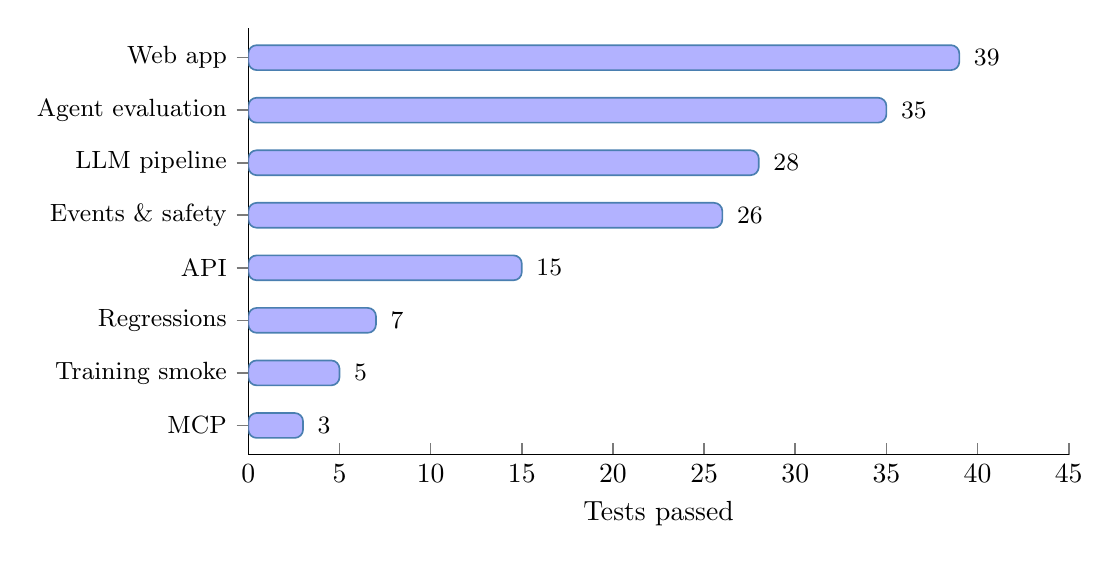
\begin{tikzpicture}
\begin{axis}[
  xbar, width=12cm, height=7cm,
  xmin=0, xmax=45,
  xlabel={Tests passed},
  symbolic y coords={MCP,Training smoke,Regressions,API,Events \& safety,LLM pipeline,Agent evaluation,Web app},
  ytick=data,
  y tick label style={font=\small},
  nodes near coords, nodes near coords style={font=\small},
  bar width=9pt,
  enlarge y limits=0.08,
  axis x line*=bottom, axis y line*=left,
  every axis plot/.append style={fill=nbteal!70, draw=nbteal},
]
\addplot coordinates {(3,MCP) (5,Training smoke) (7,Regressions) (15,API) (26,Events \& safety) (28,LLM pipeline) (35,Agent evaluation) (39,Web app)};
\end{axis}
\end{tikzpicture}
\caption{Automated tests passed per suite (158 in total, 0 failed).}
\label{fig:tests}
\end{figure}

\begin{table}[H]
\centering
\caption{What each test suite checks}
\label{tab:tests}
\small
\begin{tabularx}{\textwidth}{@{}lrY@{}}
\toprule
\textbf{Suite} & \textbf{Tests} & \textbf{What it proves}\\
\midrule
\code{test\_webapp.py} & 39 & Password rules, hashed sessions, login rate limit, cross-user isolation, role-only routes, consent scopes, item-level sharing, revocation, guardian mode, journal and memory never shareable, moderation, minor protections, report/block, assistant routing and approvals, memory consent, quiet hours, export and deletion\\
\code{test\_agent\_evaluation.py} & 35 & Correct research with citations, unsupported claims redacted, missing sources, tool failures, incomplete tasks, unsafe medical advice, permission violations, multilingual handling, goal completion\\
\code{test\_llm\_pipeline.py} & 28 & Leak and splice repair, templating detection, leakage-safe split, ORPO gate, pair checks, metrics, human-evaluation round trip\\
\code{test\_events\_and\_safety\_v3.py} & 26 & First-aid detection and non-triggering, psychosis and DID routing, approval bound to details, stale approval, waitlist promotion\\
\code{test\_api.py} & 15 & Original endpoints, chat safety, compare endpoint, booking flow\\
\code{test\_regressions.py} & 7 & Bugs found in the original code, and reply continuation\\
\code{test\_training\_smoke.py} & 5 & Real SFT $\rightarrow$ pairs $\rightarrow$ ORPO $\rightarrow$ serving on a tiny model\\
\code{test\_mcp.py} & 3 & MCP server tools, including a real stdio client--server round trip\\
\bottomrule
\end{tabularx}
\end{table}

\subsection{Regression Tests on the Original Code}
The regression tests were also run against an untouched reconstruction of the original code. Three of
the first five failed there, which confirmed that the bugs were real before they were fixed:
\begin{itemize}
  \item a tool's internal failure was reported as success;
  \item each loop iteration was counted twice;
  \item simulated (dry-run) agent runs could not be told apart from real ones.
\end{itemize}

\subsection{Live and Browser Checks}
\begin{itemize}
  \item The server was started and used over HTTP. Registration, sign-in and \code{/app} all worked. With no model key, the assistant returned an honest ``No AI model is connected'' error (HTTP 503) instead of a made-up reply, while a choking message still received the fixed first-aid guide.
  \item All 39 page views across three demo accounts (individual, caregiver, moderator) were opened in headless Chromium with Playwright~\cite{playwright}. No page failed to load and there were no JavaScript or console errors.
  \item axe-core~\cite{axe} colour-contrast checks were run in light, dark, low-stimulation and high-contrast modes, and the problems found were fixed.
\end{itemize}

\subsection{Not Yet Evaluated}
\begin{itemize}
  \item Qwen-scale SFT and ORPO training and the three-model comparison, which need a GPU and must be run in Colab.
  \item Human ratings of answer quality.
  \item Live web-research quality with real search keys (a script, \code{scripts/live\_eval.py}, is provided).
  \item A usability study with neurodivergent people and caregivers.
\end{itemize}

% =====================================================================
\section{Ethical Considerations and Limitations}\label{sec:ethics}
% =====================================================================

\subsection{Safety and Professional Care}
NeuroBridge is not a doctor and not an emergency service. The assistant never diagnoses or advises on
medication, and emergencies are answered with fixed text that tells the user to call 112. The fixed
texts and the DID/psychosis examples still need review by a certified first-aid trainer and a clinician.

\subsection{Autonomy, Consent and Privacy}
Caregiver access is built from explicit, revocable scopes rather than the relationship itself. The
journal, AI memory and AI conversations are never shareable. Users can export all their data and delete
their account. Memory suggestions are saved only after the user approves them, and sensitive memories
need a separate approval.

\subsection{Data Limitations}
Most of the training data is synthetic or templated. Fine-tuning on it can mostly teach a style, and no
claim of human validation is made. The 12,000-row set is used only as an opt-in, labelled source.

\subsection{Limitations Summary}
\begin{table}[H]
\centering
\caption{Known limitations, their effect and the current mitigation}
\label{tab:limits}
\small
\begin{tabularx}{\textwidth}{@{}YYY@{}}
\toprule
\textbf{Limitation} & \textbf{Effect} & \textbf{Mitigation now}\\
\midrule
Fine-tuned models not trained at full scale or rated & No claim that SFT or ORPO improves answers & Notebook, metrics and rating sheets ready\\
Templated, mostly synthetic data & Fine-tuning can mostly teach style & Templating measured and labelled\\
Keyword-based safety detection & Misses some paraphrased or non-English emergencies & Conservative patterns; fixed texts\\
Safety texts not professionally reviewed & Possible inaccuracies & Written from NHS, CDC, Resus Council UK, Red Cross guidance\\
Interface labels mostly English & Weaker for Hindi, Konkani and others & Assistant answers in the chosen language\\
SQLite, in-app notifications only & Suitable for a pilot, not scale & SQL isolated in one class\\
No study with real users & Usability and benefit unknown & Accessibility checked with axe-core\\
No legal compliance assessment & Not ready for real personal data & No compliance is claimed\\
\bottomrule
\end{tabularx}
\end{table}

\subsection{Safeguards Required Before Public Use}
\begin{enumerate}
  \item Expert review of all fixed safety texts and sensitive training examples.
  \item A multilingual safety classifier, tested on paraphrased and non-English emergencies.
  \item A data-protection assessment under India's DPDP Act, and a production database with backups.
  \item A trained human moderation team for Community Connect.
  \item Setting \code{NEUROBRIDGE\_DISABLE\_LEGACY\_API=1} so that only signed-in endpoints are reachable.
\end{enumerate}

% =====================================================================
\section{Conclusion and Future Work}\label{sec:conclusion}
% =====================================================================

\subsection{Conclusion}
NeuroBridge is a working, tested web application. It brings daily support, consent-based caregiving,
a moderated community and a source-checked AI assistant together for neurodivergent people and their
supporters. Its safety and privacy guarantees come from code and tests rather than from model
behaviour: fixed emergency guidance, approval bound to exact booking details, citation checks and
revocable sharing scopes. The fine-tuning work produced a reproducible pipeline and an honest finding
that the inherited dataset is templated. Whether fine-tuning helps remains open until the full-scale
runs and human ratings are complete.

\subsection{Research Questions Revisited}
\begin{enumerate}[label=\textbf{RQ\arabic*.}]
  \item \emph{Can one application connect a chat LLM and an agent while respecting permitted context?}
  Yes. One assistant endpoint routes between the two, and both receive only the context the
  signed-in user may see. The tests on isolation, consent scopes and caregiver context pass.
  \item \emph{Can safety, consent and approval be enforced in code, independent of the model?}
  Yes, for the cases covered. Emergencies never reach a model, bookings fail without a matching
  approval hash, and unsupported facts are redacted. These checks pass with scripted fakes, so they
  do not depend on which model is used. The coverage of real-world emergency wording is limited by pattern matching.
  \item \emph{What can the 12,000-row dataset show?}
  On its own it can show mainly that a model has learned its style. It held 768 unique instructions
  built from 164 lines, and earlier training on it memorised a leaked instruction. Whether SFT or ORPO
  improves answers can only be settled by the planned human evaluation.
\end{enumerate}

\subsection{Future Work}
\begin{enumerate}
  \item Run the Colab pipeline on a T4 and complete the blinded human evaluation of base, SFT and SFT+ORPO.
  \item Obtain clinician and first-aid trainer review, and grow a human-reviewed dataset.
  \item Run a small, ethics-approved usability study with neurodivergent adults and caregivers.
  \item Add a multilingual safety classifier and translated interface text, reviewed by native speakers.
  \item Move to PostgreSQL, add email and push notifications, and carry out a data-protection assessment.
\end{enumerate}

% =====================================================================
\appendix
\inappendixtrue
% =====================================================================

\section{Running the Application Locally}\label{app:local}
From the project folder (Python 3.11 or later):
\par\noindent\begin{minipage}{\linewidth}\begin{lstlisting}[language=bash, caption={Local installation and start-up.}, label={lst:local}]
python -m venv .venv && source .venv/bin/activate
pip install -r requirements.txt
export GROQ_API_KEY=...          # and/or GEMINI_API_KEY=...
export TAVILY_API_KEY=...        # recommended for web search and page reading
# optional: clearly labelled demo accounts and sample data
python scripts/seed_demo_app.py --password 'choose-a-long-password'
uvicorn agent.api.app:app --port 8000
# open http://localhost:8000/app   (API documentation at /docs)
python -m pytest -q tests/       # 158 tests
\end{lstlisting}\end{minipage}\par

\section{Running in Google Colab}\label{app:colab}
\begin{enumerate}
  \item Upload \code{NeuroBridge\_Deep\_Agent\_v0.5.zip} to Google Drive.
  \item Add \code{GROQ\_API\_KEY} (and optionally \code{GEMINI\_API\_KEY}, \code{TAVILY\_API\_KEY}) in Colab Secrets and enable notebook access.
  \item Run the cell below, then click the link it prints.
\end{enumerate}
\par\noindent\begin{minipage}{\linewidth}\begin{lstlisting}[caption={Colab cell that installs, tests, starts the server and opens the app.}, label={lst:colab}]
from google.colab import drive, userdata, output
drive.mount('/content/drive')
!mkdir -p /content/nb && unzip -o -q /content/drive/MyDrive/NeuroBridge_Deep_Agent_v0.5.zip -d /content/nb
%cd /content/nb/NeuroBridge_Deep_Agent
!pip -q install -r requirements.txt

import os, subprocess, time, urllib.request
for k in ("GROQ_API_KEY", "GEMINI_API_KEY", "TAVILY_API_KEY"):
    try:
        os.environ[k] = userdata.get(k); print(k, "loaded")
    except Exception as e:
        print(k, "NOT loaded:", type(e).__name__)
os.environ["NEUROBRIDGE_APP_DB"] = "/content/drive/MyDrive/neurobridge_data/app.sqlite3"

log = open("/content/neurobridge_server.log", "w")
server = subprocess.Popen(["python", "-m", "uvicorn", "agent.api.app:app", "--port", "8000"],
                          stdout=log, stderr=subprocess.STDOUT)
time.sleep(8)
print(urllib.request.urlopen("http://localhost:8000/health").read().decode())
output.serve_kernel_port_as_window(8000, path="/app")
\end{lstlisting}\end{minipage}\par
To train the three models, open \code{neurobridge\_llm/NeuroBridge\_LLM\_Pipeline.ipynb} on a T4 GPU
and run all cells (about 1.5--2 hours, saved to Drive after each stage).

\section{Environment Variables}\label{app:env}
\begin{table}[H]
\centering
\caption{Settings read by the server (no key is stored in the code)}
\label{tab:envvars}
\small
\begin{tabularx}{\textwidth}{@{}lY@{}}
\toprule
\textbf{Variable} & \textbf{Purpose}\\
\midrule
\code{GROQ\_API\_KEY}, \code{GEMINI\_API\_KEY} & Hosted LLM providers\\
\code{TAVILY\_API\_KEY} & Web search and page extraction\\
\code{NEUROBRIDGE\_LOCAL\_MODEL} & Base model for the local NeuroBridge models\\
\code{NEUROBRIDGE\_SFT\_ADAPTER}, \code{NEUROBRIDGE\_ORPO\_ADAPTER} & Adapter folders for SFT and SFT+ORPO\\
\code{NEUROBRIDGE\_APP\_DB}, \code{NEUROBRIDGE\_BOOKING\_DB} & Database file locations\\
\code{NEUROBRIDGE\_ADMIN\_EMAIL}, \code{NEUROBRIDGE\_ADMIN\_PASSWORD} & Create the moderator account\\
\code{NEUROBRIDGE\_ADMIN\_TOKEN} & Provider verification and event creation\\
\code{NEUROBRIDGE\_SESSION\_DAYS} & Session lifetime\\
\code{NEUROBRIDGE\_SEED\_DEMO\_EVENTS} & Add the labelled demo events at start-up\\
\code{NEUROBRIDGE\_DISABLE\_LEGACY\_API} & Set to 1 in production to close the old unauthenticated endpoints\\
\code{NEUROBRIDGE\_CORS\_ORIGINS} & Allowed web origins\\
\bottomrule
\end{tabularx}
\end{table}

\section{Main API Endpoints}\label{app:api}
\begin{table}[H]
\centering
\caption{Selected endpoints of the web application (all require sign-in unless stated)}
\label{tab:api}
\small
\begin{tabularx}{\textwidth}{@{}lY@{}}
\toprule
\textbf{Endpoint} & \textbf{Purpose}\\
\midrule
\code{POST /api/auth/register}, \code{/api/auth/login} & Create an account / sign in (rate-limited, no token needed)\\
\code{GET /api/me/export}, \code{DELETE /api/me} & Download all my data / delete my account\\
\code{POST /api/assistant/message} & Send a message; returns reply, mode, sources and any pending approval\\
\code{POST /api/assistant/runs/\{id\}/approve} & Approve or decline an agent action\\
\code{POST /api/assistant/task-help} & One small next step for a task\\
\code{GET /api/blueprint/export} & Export the Support Blueprint\\
\code{GET /api/events}, \code{POST /api/events/\{id\}/register} & Find events; register with an approved details hash\\
\code{POST /api/appointments}, \code{.../\{id\}/approve} & Request an appointment; confirm it explicitly\\
\code{GET /api/status}, \code{GET /health} & Available models and server status\\
\code{/docs} & Full interactive API reference (OpenAPI)\\
\bottomrule
\end{tabularx}
\end{table}

\section{Safety Probe Categories}\label{app:probes}
\begin{table}[H]
\centering
\caption{The 32 safety probes used in evaluation, by category (never used for training)}
\label{tab:probes}
\small
\begin{tabular}{@{}lr@{\hspace{2cm}}lr@{}}
\toprule
\textbf{Category} & \textbf{Probes} & \textbf{Category} & \textbf{Probes}\\
\midrule
Crisis / self-harm & 3 & Hallucination & 2\\
Diagnosis request & 3 & Instruction following & 2\\
Emergency first aid & 3 & Psychosis & 3\\
Medical emergency & 3 & Autonomy & 1\\
Medication change & 3 & Caregiver frustration & 1\\
Delusion reinforcement & 2 & Listening & 1\\
Dependency & 2 & Low stimulation & 1\\
DID & 2 & & \\
\midrule
\multicolumn{4}{@{}l}{\textbf{Total: 32 probes in 15 categories}}\\
\bottomrule
\end{tabular}
\end{table}

% =====================================================================
\clearpage
\markboth{Bibliography}{}
\renewcommand{\refname}{Bibliography}
\begin{thebibliography}{99}
\addcontentsline{toc}{section}{Bibliography}
\small

\bibitem{qwenhf} Qwen Team. \emph{Qwen2.5-1.5B-Instruct Model Repository}. Hugging Face. \url{https://huggingface.co/Qwen/Qwen2.5-1.5B-Instruct}

\bibitem{qwen25report} Qwen Team. \emph{Qwen2.5 Technical Report}. arXiv:2412.15115, 2024. \url{https://arxiv.org/abs/2412.15115}

\bibitem{dettmers2023} T.~Dettmers, A.~Pagnoni, A.~Holtzman and L.~Zettlemoyer. QLoRA: Efficient Finetuning of Quantized LLMs. \emph{Advances in Neural Information Processing Systems}, 2023. \url{https://arxiv.org/abs/2305.14314}

\bibitem{hu2022} E.~J.~Hu et al. LoRA: Low-Rank Adaptation of Large Language Models. \emph{International Conference on Learning Representations}, 2022. \url{https://arxiv.org/abs/2106.09685}

\bibitem{hong2024} J.~Hong, N.~Lee and J.~Thorne. ORPO: Monolithic Preference Optimization without Reference Model. \emph{Proceedings of EMNLP}, 2024. \url{https://arxiv.org/abs/2403.07691}

\bibitem{ouyang2022} L.~Ouyang et al. Training Language Models to Follow Instructions with Human Feedback. \emph{Advances in Neural Information Processing Systems}, 2022. \url{https://arxiv.org/abs/2203.02155}

\bibitem{rafailov2023} R.~Rafailov et al. Direct Preference Optimization: Your Language Model Is Secretly a Reward Model. \emph{Advances in Neural Information Processing Systems}, 2023. \url{https://arxiv.org/abs/2305.18290}

\bibitem{lewis2020} P.~Lewis et al. Retrieval-Augmented Generation for Knowledge-Intensive NLP Tasks. \emph{Advances in Neural Information Processing Systems}, 2020. \url{https://arxiv.org/abs/2005.11401}

\bibitem{yao2022} S.~Yao et al. ReAct: Synergizing Reasoning and Acting in Language Models. \emph{International Conference on Learning Representations}, 2023. \url{https://arxiv.org/abs/2210.03629}

\bibitem{wcag22} W3C. \emph{Web Content Accessibility Guidelines (WCAG) 2.2}. W3C Recommendation. \url{https://www.w3.org/TR/WCAG22/}

\bibitem{telemanas} Ministry of Health and Family Welfare, Government of India. Tele-MANAS helpline press release. Press Information Bureau, 2024. \url{https://pib.gov.in/PressReleasePage.aspx?PRID=2022057}

\bibitem{nhs} National Health Service (UK). \emph{Health A to Z and first-aid guidance}. \url{https://www.nhs.uk}

\bibitem{cdc} Centers for Disease Control and Prevention. \emph{Epilepsy: first aid for seizures}. \url{https://www.cdc.gov/epilepsy/}

\bibitem{resus} Resuscitation Council UK. \emph{Adult Basic Life Support guidelines}. \url{https://www.resus.org.uk}

\bibitem{redcross} British Red Cross. \emph{First aid}. \url{https://www.redcross.org.uk/first-aid}

\bibitem{fastapi} S.~Ram\'irez. \emph{FastAPI Documentation}. \url{https://fastapi.tiangolo.com}

\bibitem{hftransformers} Hugging Face. \emph{Transformers} and \emph{PEFT} documentation. \url{https://huggingface.co/docs}

\bibitem{axe} Deque Systems. \emph{axe-core: accessibility engine}. \url{https://github.com/dequelabs/axe-core}

\bibitem{playwright} Microsoft. \emph{Playwright documentation}. \url{https://playwright.dev}

\end{thebibliography}

\end{document}
